%====================Kapitola:Elektrostatika==================================================================
\chapter{Elektrostatika}\label{chap:fey_electrostatics}
\minitoc
\newpage
  %------------------------ Statika -----------------------------------------------------------------
  \section{Statika}
    \cite[s.~63]{Feynman02} Nyní začněme s podrobným studiem teorie elektromagnetizmu. Celý     
    elektromagnetizmus je obsažen v Maxwellových rovnicích.
    
    \emph{Maxwellovy rovnice:}
    \begin{align}\label{fyz:fey_eq_elstat01}
      \ndiver{E} &=  \frac{\varrho}{\varepsilon_0}                     \\
        \nrot{E} &= -\pder{\vec{B}}{t}                                 \\
     c^2\nrot{B} &=  \pder{\vec{E}}{t} + \frac{\vec{j}}{\varepsilon_0} \\
      \ndiver{B} &= 0.                               
    \end{align}
     
    Situace popsané těmito rovnicemi mohou být velice složité. Nejdříve budeme uvažovat o poměrně
    jednoduchých situacích a učit se, jak s nimi zacházet. Složitější situace probereme až potom. 
    Nejsnáze se pracuje ve statickém případě\footnote{Vlastně stacionárním případě. O elektrostatice 
    mluvíme obyčejně tehdy, když jsou náboje nehybné.}, kdy nic nezávisí na čase. Tehdy mají všechny
    náboje trvale pevnou polohu v prostoru anebo, pohybují-li se, pak pouze jako ustálený proud v 
    obvodu (takže se \(\varrho\) a \(\vec{j}\) v čase nemění). V těchto podmínkách všechny členy, 
    které jsou časovými derivacemi pole, jsou rovny nule a Maxwellovy rovnice získají tento tvar:
     
    \begin{align}
     \shortintertext{\emph{Elektrostatika:}} 
      \ndiver{E} &=  \frac{\varrho}{\varepsilon_0}    \label{fyz:fey_eq_elstat02a}   \\  
        \nrot{E} &= 0                                 \label{fyz:fey_eq_elstat02b}   \\
      \shortintertext{\emph{Magnetostatika:}}  
        \nrot{B} &=  \frac{\vec{j}}{\varepsilon_0c^2} \label{fyz:fey_eq_elstat02c}   \\
      \ndiver{B} &= 0.                                \label{fyz:fey_eq_elstat02d}
    \end{align}    
     
    Na soustavě těchto čtyř rovnic si všimněte zajímavé věci. Soustavu lze rozdělit na dva páry 
    rovnic. Přitom elektrické pole \(\vec{E}\) se objevuje pouze v prvních dvou a magnetické pole 
    \(\vec{B}\) pouze v druhých dvou rovnicích soustavy. Obě pole spolu vzájemně nesouvisí. Znamená 
    to, že \emph{dokud jsou proudy a náboje statické, jsou elektřina a magnetizmus oddělené jevy}. 
    Vzájemná závislost \(\vec{E}\) a \(\vec{B}\) se neobjeví, pokud nedochází k takovým změnám 
    nábojů anebo proudů jako při nabíjení kondenzátoru anebo při pohybu magnetu. \(\vec{E}\) a 
    \(\vec{B}\) budou na sobě navzájem záviset pouze v případě dostatečně rychlých změn, když v 
    Maxwellových rovnicích dostanou význam časové derivace.
     
    Podíváte-li se na rovnice statiky, uvidíme, že studium obou těchto předmětů, které nazýváme     
    elektrostatika a magnetostatika, je ideální pro seznámení se s matematickými vlastnostmi 
    vektorových polí. Elektrostatika je čistým příkladem vektorového pole s \emph{nulovou rotací a 
    nenulovou divergencí}. Magnetostatika je čistým příkladem pole s \emph{nulovou divergencí a 
    nenulovou rotaci}. Častější, a snad si myslíte, že i lepší, způsob přednášení teorie 
    elektromagnetizmu je začít nejdřív elektrostatikou, a tak se poučit o divergenci. Magnetostatika 
    a rotace budou probrány později. Poté se elektřina a magnetizmus spolu zkombinují. My jsme se 
    rozhodli, začít úplnou teorií vektorového počtu. Nyní ji budeme aplikovat na speciální případ, 
    na elektrostatiku, tj. na pole \(\vec{E}\) dané prvním párem rovnic (\ref{fyz:fey_eq_elstat02a}) 
    a (\ref{fyz:fey_eq_elstat02b}).
     
    Začněme nejjednoduššími situacemi, tedy těmi, v nichž jsou dány polohy všech nábojů. Kdybychom 
    měli studovat elektrostatiku pouze na této úrovni (což budeme dělat ve dvou následujících 
    kapitolách), bylo by to velmi jednoduché, téměř banální. Jak uvidíte, vše je možné získat z 
    Coulombova zákona a  několika integrací. V mnoha reálných elektrostatických úlohách však 
    zpočátku nevíme, kde náboje jsou. Víme pouze, že se mezi sebou rozdělily podle vlastností látky. 
    Polohy, jež náboje zaujaly, závisí na poli \(\vec{E}\), a to zase závisejí na polohách nábojů. 
    Tím se věci značně komplikují. Umístíme-li například do blízkosti vodiče nebo izolátoru nabité 
    těleso, elektrony a protony ve vodiči nebo v izolátoru se přemístí. Hustota náboje \(\varrho\) v 
    rovnici (\ref{fyz:fey_eq_elstat02a}) pak bude mít jednu část, kterou určíme z velikosti 
    přeneseného náboje, ale i další části, pocházející od nábojů, které se přemístily ve vodiči. Je 
    nutné započítat všechny náboje. Přitom je možné dospět k některým záludným a zajímavým 
    problémům. Ačkoli se má tato kapitola zabývat elektrostatikou, její hezčí a náročnější partie 
    neobsáhne. Budeme v ní rozebírat situaci, kdy polohy všech nábojů můžeme pokládat za známé. 
    Přirozeně, měli byste být schopni zvládnout tuto situaci dřív, než se pokusíte řešit složitější 
    problémy.
    
  % ----------------- Coulombův zákon, superpozice --------------------------------------------------
  \section{Coulombův zákon, superpozice}  
    \cite[s.~65]{Feynman02} Bylo by logické vyjít z rovnic (\ref{fyz:fey_eq_elstat02a}) a 
    (\ref{fyz:fey_eq_elstat02b}).Jednodušší však bude, začneme-li někde jinde a vrátíme se k těmto 
    rovnicím. Výsledky budou ekvivalentní. Začneme zákonem, o němž jsme již hovořili dříve, tzv. 
    \emph{Coulombovým zákonem}. Podle něho působí mezi dvěma nepohybujícími se náboji síla, která je 
    přímo úměrná součinu nábojů a nepřímo úměrná druhé mocnině vzdálenosti mezi nimi. Síla má směr 
    přímky spojující oba náboje.
    \begin{equation}\label{fyz:fey_eq_elstat09}
     \text{\emph{Coulombův zákon}} \qquad 
       \vec{F}_1=\frac{1}{4\pi\varepsilon_0}\frac{q_1q_2}{r_{12}^2}\vec{e}_{12} = \vec{F}_2,
    \end{equation}
    kde \(\vec{F}_1\) je síla působící na náboj \(q_1\), \(e_{12}\) je jednotkový vektor směřující 
    od \(q_2\) k \(q_1\) a \(r_{12}\) je vzdálenost mezi \(q_2\) k \(q_1\). Síla \(\vec{F}_2\) 
    působící na náboj \(q_2\) je stejně velká jako \(\vec{F}_1\), ale má opačný směr.
     
    Konstanta úměrnosti se z historických důvodů píše jako \(\frac{1}{4\pi\varepsilon_0}\). V 
    soustavě jednotek SI, kterou používáme, je rovna přesně \(10^{-7}c^2\) (\num{10e-7}-krát druhá 
    mocnina rychlosti světla ve vakuu). Protože rychlost světla ve vakuu je přibližně 
    \SI{10e8}{\meter\per\second}, konstanta má hodnotu zhruba \SI{9e9}{\meter\per\farad} 
    (metr/farad) a její rozměr vzhledem k základním veličinám soustavy SI je 
    \si{\cubic\meter\kilogram\second^{-4}\ampere^{-2}}.
    \begin{alignat*}{3}
     &\frac{1}{4\pi\varepsilon_0} &&= 10^{-7}c^2   \qquad && \ldots \text{z definice}     \\
     &                            &&= 9,0\cdot10^9 \qquad && \ldots \text{z experimentu} 
    \end{alignat*}
    Možné způsoby vyjádření rozměru konstanty jednotky: 
    \begin{itemize}
     \setlength{\itemsep}{0cm}%
     \setlength{\parskip}{0em}%
       \item \si{\meter\per\farad},    
       \item nebo \si{\newton\square\meter\per\square\coulomb},    
       \item nebo \si{\cubic\meter\kilogram\second^{-4}\ampere^{-2}},
       \item nebo \si{\volt\meter\per\coulomb}.
    \end{itemize}
    
    Jde-li o víc než dva náboje - a pouze takové případy jsou opravdu zajímavé - musíme Coulombův 
    zákon doplnit ještě jedním přírodním zákonem: síla působící na jakýkoliv náboj je vektorovým 
    součtem Coulombových sil pocházejících od všech ostatních nábojů. Tento zákon se nazývá 
    \emph{princip superpozice}. To je vše, co se týká elektrostatiky. Kombinujeme-li Coulombův 
    zákon a princip superpozice, není nic víc třeba. Rovnice (\ref{fyz:fey_eq_elstat02a}) a 
    (\ref{fyz:fey_eq_elstat02b}) - rovnice elektrostatiky - neříkají nic více, nic méně.
     
    Při používání Coulombova zákona je vhodné zavést pojem elektrického pole. Říkáme, že pole 
    \(\vec{E}(1)\) je rovno síle působící na náboj \(q_1\) (ze strany všech ostatních nábojů) a 
    připadající \emph{na jednotku náboje} (tj. vektor působící síly, dělený velikostí náboje 
    (\(q_1\)). Vydělíme-li rovnost (\ref{fyz:fey_eq_elstat09}) (\(q_1\)), dostaneme pro účinek 
    nábojů jiných než (\(q_1\)), že
    \begin{equation}\label{fyz:fey_eq_elstat11}
     \vec{E}(1) = \frac{1}{4\pi\varepsilon_0}\frac{q_2}{r^2_{12}}\vec{e}_{12}
    \end{equation}
    Chápeme to tak, že \(\vec{E}(1)\) udává cosi pro bod \(1\) i tehdy, kdyby tam náboj \(q_1\) 
    nebyl -  za předpokladu, že všechny ostatní náboje zachovají své původní polohy. Říkáme, že 
    \(\vec{E}(1)\) je elektrické pole v bodě \(1\).
     
    Elektrické pole \(\vec{E}(1)\) je vektor, takže rovnicí (\ref{fyz:fey_eq_elstat11}) myslíme ve 
    skutečnosti tři rovnice pro  každou složku jednu. Explicitně vypíšeme x-ovou složku, pro kterou 
    z rovnice (\ref{fyz:fey_eq_elstat11}) vyplývá, že
      \begin{equation}\label{fyz:fey_eq_elstat12}
      E_x(x,y,z) = \frac{q_2}{4\pi\varepsilon_0}
                   \frac{x_1-x_2}{[(x_1-x_2)^2+(y_1-y_2)^2+(z_1-z_2)^2]^{\frac{3}{2}}}
    \end{equation}
    Podobně pro ostatní složky.
     
    Je-li víc nábojů, je pole \(\vec{E}\) v nějakém bodě \(1\) součtem příspěvků od každého z 
    ostatních nábojů. Každý člen součtu bude mít tvar (\ref{fyz:fey_eq_elstat11}), resp. 
    (\ref{fyz:fey_eq_elstat12}). Bude-li \(q_j\) označovat velikost \(j\)-tého náboje a  
    \(\vec{r}_{1j}\) je vektor posunutí z polohy 
    \(q_j\) do bodu \(1\), píšeme
    \begin{align}
      \vec{E}(1) &= \sum\limits_{j=1}\frac{1}{4\pi\varepsilon_0}\frac{q_j}{r^2_{1j}}\vec{e}_{1j}
                    \label{fyz:fey_eq_elstat13}    \\
      \shortintertext{což, samozřejmě, znamená, že}
      E_x(x,y,z) &= \sum\limits_{j=1}\frac{q_j}{4\pi\varepsilon_0}
                    \frac{x_1-x_j}{[(x_1-x_j)^2+(y_1-y_j)^2+(z_1-z_j)^2]^{\frac{3}{2}}} 
                    \label{fyz:fey_eq_elstat14}    
      \shortintertext{a analogicky pro další složky.}  \nonumber
    \end{align}     
    
    \vspace{-3em}
    Často je pohodlnější nebrat v úvahu fakt, že náboje existují jako diskrétní objekty - protony a 
    elektrony - a pokládat je za rozptýlené v nějakém spojitém útvaru anebo, jak se to nazývá, v 
    nějakém „rozdělení“. Tento přístup je v pořádku, pokud nás nezajímá, co se děje ve velmi malých 
    rozměrech. Rozdělení náboje charakterizujeme „\emph{hustotou náboje}“ \(\varrho(x, y, z)\). 
    Nachází-Ii se v malém objemu \(\Delta V_2\) v okolí bodu \(2\) množství náboje \(\Delta q_2\), 
    pak je \(\varrho\) definováno vztahem
    \begin{equation}\label{fyz:fey_eq_elstat15}
     \Delta q_2 = \varrho(2)\Delta V_2.
    \end{equation}
    \begin{figure}[ht!]
      \centering
      \includegraphics[width=0.7\linewidth]{fey_el_pole.jpg}
      \caption{Elektrické pole \(\vec{E}_v\) bodě \(1\) nějakého rozdělení nábojů získáme 
               integrálem přes toto rozdělení. Bod \(1\) se může nacházet i uvnitř rozdělení}
    \end{figure}
    Při používání Coulombova zákona při takovém přístupu nahradíme sumy ve vztazích 
    (\ref{fyz:fey_eq_elstat13}) a (\ref{fyz:fey_eq_elstat14}) integrály přes všechny objemy 
    obsahující náboje. Pak bude platit
    \begin{equation}\label{fyz:fey_eq_elstat16}
      \vec{E}(1) = \bigints\limits_{\substack{\text{celý}\\\text{prostor}}}
                       \frac{1}{4\pi\varepsilon_0}
                       \frac{\varrho(2)\vec{e}_{12}}{r^2_{12}}\dd{V_2}
    \end{equation}
    Někteří lidé píšou raději     
    \begin{equation*}
      \vec{e}_{12} = \frac{\vec{r}_{12}}{r_{12}}
    \end{equation*}
    kde \(\vec{r}_{12}\) je vektor posunutí z \(2\) do\(1\) (obr. \ref{FYZ:fig_fey_potencial1}). 
    Integrál udávající \(\vec{E}\) je pak zapsán takto
    \begin{equation}\label{fyz:fey_eq_elstat17}
      \vec{E}(1) = \bigints\limits_{\substack{\text{celý}\\\text{prostor}}}
                       \frac{1}{4\pi\varepsilon_0}
                       \frac{\varrho(2)\vec{r}_{12}}{r^3_{12}}\dd{V_2}
    \end{equation}
    Chceme-li pomocí těchto integrálů něco vypočítat, musíme je obvykle podrobně rozepsat. Pro 
    \(x\)-ovou složku rovností (\ref{fyz:fey_eq_elstat16}) nebo (\ref{fyz:fey_eq_elstat17}) bychom 
    pak psali        
    \begin{widetext}
      \begin{equation}\label{fyz:fey_eq_elstat18}
        E_x(x_1, y_1, z_1) = 
          \frac{1}{4\pi\varepsilon_0}
          \bigints\limits_{\substack{\text{celý}\\\text{prostor}}}\varrho(x_2, y_2, z_2)          
          \frac{x_1-x_2}{[(x_1-x_2)^2+(y_1-y_2)^2+(z_1-z_2)^2]^{\frac{3}{2}}}\dd{x_2}\dd{y_2}\dd{z_2}
      \end{equation}  
    \end{widetext} 
%
    Tento vzorec nebudeme používat často. Napsali jsme jej sem pouze proto, abychom zdůraznili 
    fakt, že jsme úplně vyřešili všechny ty elektrostatické úlohy, ve kterých známe polohy všech 
    nábojů. Jsou dány náboje. Jaká jsou pole? Odpověď: vypočtěte tento integrál. Nic víc k tomu není 
    potřeba; pouze výpočet složitých trojrozměrných integrálů - přesně vzato, je to práce pro 
    počítač.
    
    Pomocí našich integrálů můžeme najít pole vytvářená nabitým rovinným nebo lineárním útvarem, 
    nabitou kulovou plochou anebo jiným udaným rozdělením náboje. Je důležité uvědomit si, že i 
    když budeme kreslit siločáry, hovořit o potenciálech nebo počítat divergence, výsledek už máme. 
    Závisí pouze na tvaru tohoto integrálu. Někdy je snadnější jej vypočítat nějakým důvtipným 
    trikem než jeho skutečným výpočtem. Ovládat takovéto postupy však vyžaduje naučit se mnohé 
    neobyčejné věci. V praxi je možná jednodušší nesnažit se dělat chytrého, a namísto toho 
    vypočítat vždy integrál přímo. I přesto se však nyní pokusíme být v této záležitosti důvtipnými 
    a budeme pokračovat analýzou některých jiných vlastností elektrického pole.     

  %------------------------ Elektrický potenciál ----------------------------------------------------
  \section{Elektrický potenciál}
    \cite[s.~66]{Feynman02} Nejdříve probereme pojem elektrického potenciálu, který souvisí s prací 
    vykonanou při přenášení náboje z jednoho bodu do druhého. Mějme nějaké rozdělení náboje, které 
    vytváří elektrické pole. Ptejme se, kolik práce je třeba vynaložit na přenos malého náboje z 
    jednoho místa na druhé. Práce, která se vykonává přenášením náboje po nějaké dráze proti 
    elektrickým silám, je rovna záporně vzatému integrálu po této dráte ze složky elektrické síly ve 
    směru pohybu. 
     
    Přenášíme-li náboj z bodu \(a\) do bodu \(b\), bude platit
    \begin{equation*}
      W = -\int_{a}^{b}\vec{F}\dd{\vec{s}},
    \end{equation*}
    kde \(\vec{F}\) je elektrická síla působící na náboj v každém bodě a \(\dd{\vec{s}}\) je 
    diferenciální vektor posunutí podél dráhy (obr. \ref{FYZ:fig_fey_potencial1}).
    
    Pro naše účely je zajímavější uvažovat práci, která by se konala při přenášení jedné jednotky 
    náboje. Tehdy síla působící na náboj je číselně rovna intenzitě elektrického pole. Označíme-li 
    práci vykonanou proti elektrickým silám v tomto případě \(W_{jedn}\) můžeme psát
    \begin{equation}\label{fyz:fey_eq_elstat19}
      W_{jedn} = -\int_{a}^{b}\vec{E}\dd{\vec{s}}.
    \end{equation}
    
    To, co dostaneme pomocí takového integrálu, obecně závisí na dráze, po které integrujeme. 
    Jestliže by integrál (\ref{fyz:fey_eq_elstat19}) závisel na dráze od \(a\) do \(b\), mohli 
    bychom z pole získávat práci přenášením náboje do \(b\) po jedné dráze a pak zpět do \(a\) po 
    jiné. Do \(b\) bychom šli po dráze, pro kterou je \(W\) menší, a \emph{zpět} po jiné dráze, 
    odčerpávající \emph{víc} práce, \emph{než} vkládáme.
    
    Získávat energii z pole - na tom není v principu nic nemožného. Opravdu se setkáme s poli, kde 
    to možné je. Může se stát, že když pohybujete nábojem, působíte silami na jinou část 
    „mechanizmu“. Pohybuje-li se mechanizmus proti síle, ztrácí energii, přičemž celková energie v 
    přírodě se nemění. Avšak v elektrostatice takový „mechanizmus“ není. Víme, jaké síly působí 
    zpětně na zdroje pole. Jsou to coulombovské síly působící na náboje, které jsou původci pole. 
    Mají-li Ostatní náboje v prostoru pevné polohy, což předpokládáme pouze v elektrostatice, 
    nevykonávají tyto zpětné síly při působení práci. Neexistuje žádný způsob, jak z nich získat 
    energii, samozřejmě za předpokladu, že v elektrostatických situacích platí princip zachování 
    energie. Věříme, že platí, ale teď ukážeme, že to musí vyplývat z Coulombova zákona pro 
    sílu.         
    
    \begin{figure}
      \includegraphics[width=0.8\linewidth]{fey_el_potencial1.jpg}
      \caption{Práce konaná při přenesení náboje z \(a\) do \(b\) je rovna záporně vzatému 
               integrálu ze skalárního součinu \(\vec{F}\cdot d\vec{s}\) po dráze z \(a\) do \(b\)}
      \label{FYZ:fig_fey_potencial1}
    \end{figure}
   
    Uvažujme nejdříve, co se stane v poli vyvolaném jediným nábojem \(q\), Nechť je bod \(a\) ve 
    vzdálenosti \(r_1\) od \(q\) a bod \(b\) ve vzdálenosti \(r_2\). Nyní z \(a\) do \(b\) přenesme 
    jiný náboj, který budeme nazývat „zkušebním“ nábojem a jehož velikost zvolíme rovnou jedné 
    jednotce. Začněme s tou dráhou, která je ze všech možných drah pro výpočet nejjednodušší. Náš 
    zkušební náboj přeneseme nejdřív po oblouku kružnice a pak podél poloměru, jak to znázorňuje 
    obr. \ref{fyz:fig_fey_elpot2}. Najít práci vykonanou na této speciální dráze je dětskou hrou 
    (jinak bychom ji nebyli zvolili). Především vůbec žádná práce se nevykoná na dráze z \(a\) do 
    \(a'\). Pole je radiální (podle Coulombova zákona), takže jeho intenzita je kolmá na směr 
    pohybu. Dále na dráze z \(a'\) do \(b\) má intenzita pole směr pohybu a mění se jako 
    \(\frac{1}{r^2}\). Práce vykonaná přenosem zkušebního náboje z \(a\) do \(b\) bude
    \begin{equation}\label{fyz:fey_eq_elstat20}
     -\int_{a}^{b}\vec{E}\dd{\vec{s}} = 
       -\frac{q}{4\pi\varepsilon_0}\int_{a'}^{b}\frac{\dd{r}}{r^2} = 
       -\frac{q}{4\pi\varepsilon_0}\left(\frac{1}{r_{a}}-\frac{1}{r_{b}}\right).  
    \end{equation}
    \begin{figure}[ht!]
      \centering
      \begin{tabular}{c}
        \subfloat[ ]{\label{fyz:fig_fey_elpot2}
          \includegraphics[width=0.3\textwidth]{fey_el_potencial2.jpg}}              \\
        \subfloat[ ]{\label{fyz:fig_fey_elpot3} 
          \includegraphics[width=0.3\textwidth]{fey_el_potencial3.jpg}}  
      \end{tabular}
      \caption{Přenášením zkušebního náboje z a do b po obou těchto drahách se koná stejná práce}
    \end{figure}
    
    Vezměme nyní jinou jednoduchou dráhu, např. takovou, jaká je znázorněná na obr. 
    \ref{fyz:fig_fey_elpot3}. Chvíli vede po oblouku kružnice, potom chvíli radiálně, potom  opět po 
    oblouku a potom radiálně atd. Předně, když jdeme po oblouku kružnice, práci nevykonáváme. Když 
    jdeme po radiálním úseku, musíme integrovat \(\frac{1}{r^2}\). Na prvním radiálním úseku 
    integrujeme z \(r_{a}\) do \(r_{a'}\), na druhém úseku z \(r_{a'}\) do \(r_{a''}\) atd. Součet 
    všech těchto integrálů dá totéž jako jediný integrál přímo z \(r_{a}\) do \(r_{b}\). Pro tuto 
    dráhu dostáváme stejný výsledek, jaký jsme dostali v případě první dráhy. Je zřejmé, že tentýž 
    výsledek bychom dostali pro jakoukoliv dráhu, která se skládá z libovolného počtu takovýchto 
    úseků.
    
    Jak to bude v případě hladkých drah? Dostali bychom tentýž výsledek? O této otázce jsme hovořili 
    už ve 13. kapitole 1. dílu. Na základě stejných důvodů, které jsme použili tam, můžeme udělat 
    závěr, že práce vykonaná při přenášení jednotkového náboje z \(a\) do \(b\) nezávisí na dráze.   
    \begin{equation*}
      W_{\substack{\text{jedn}\\ a-b}} = 
       - \int\limits_{\substack{a\\\text{jakákoliv}\\\text{dráha}}}^b\vec{E}\dd{\vec{s}}.
    \end{equation*}      
    
    Protože vykonaná práce závisí pouze na koncových bodech, je možné ji udat jako rozdíl dvou 
    čísel. Přesvědčíme se o tom následujícím způsobem. Zvolme vztažný bod \(P_0\) a domluvme se, že 
    budeme počítat náš integrál použitím dráhy, která bude vždy procházet bodem \(P_0\). Nechť 
    \(\varphi(a)\) označuje práci vykonanou proti poli při přechodu z \(P_0\) do bodu \(a\) a 
    \(\varphi(b)\) práci vykonanou při přechodu z \(P_0\) do bodu \(b\) (obr. 
    \ref{FYZ:fig_fey_potencial4}). Práce vykonaná při přechodu z \(a\) do \(P_0\) (cestou do \(b\)) 
    je záporně vzaté \(\varphi(a)\), takže bude platit
    
    \begin{equation}\label{fyz:fey_eq_elstat21}
     - \int\limits_{a}^{b}\vec{E}\dd{\vec{s}} = \varphi(b) - \varphi(a). 
    \end{equation}
    Protože tu bude vždy vystupovat pouze rozdíl hodnot funkce \(\varphi\) ve dvou bodech, ve 
    skutečnosti nepotřebujeme ani specifikovat polohu bodu \(P_0\). Jakmile jsme však zvolili nějaký 
    referenční bod, hodnota \(\varphi\) je už určena pro každý bod v prostoru; \(\varphi\) je tedy 
    \emph{skalární pole}. Je funkcí \(x, y, z\). Tuto skalární funkci nazýváme 
    \emph{elektrostatickým potenciálem} v libovolném bodě.

    \emph{Elektrostatický potenciál:}
     \begin{equation}\label{fyz:fey_eq_elstat22}
       \varphi(P) = - \int\limits_{P_0}^{P}\vec{E}\dd{\vec{s}} = \varphi(b) - \varphi(a). 
     \end{equation} 
    
    Často je pohodlné volit vztažný	bod v nekonečnu. V případě jednotlivého	náboje nacházejícího se 
    v počátku souřadnicové soustavy pak s ohledem	na vztah (\ref{fyz:fey_eq_elstat20}) pro potenciál 
    \(\varphi\) v nějakém bodě \((x, y, z)\) dostaneme
    \begin{equation}\label{fyz:fey_eq_elstat23}
     \varphi(x, y, z) = \frac{q}{4\pi\epsilon_0}\frac{1}{r}. 
    \end{equation}

    \begin{figure}
      \centering
      \includegraphics[width=0.8\linewidth]{fey_el_potencial4.jpg}
      \caption{Práce vykonaná při postupu po jakékoliv dráze z \(a\) do \(b\) je rovna záporně     
               vzaté práci z nějakého bodu \(P_0\) do \(a\) zvětšené o práci z \(P_0\) do \(b\)}
      \label{FYZ:fig_fey_potencial4}
    \end{figure}

    Elektrické pole několika nábojů je možné napsat jako součet elektrického pole prvního, druhého, 
    třetího atd. náboje. Integrujeme-li součet, abychom našli potenciál, dostaneme součet integrálů. 
    Každý z těchto integrálů představuje potenciál jednoho z nábojů. Usuzujeme tak proto, že 
    potenciál množiny nábojů je součtem potenciálů jednotlivých nábojů. Princip superpozice platí 
    tedy i pro potenciály. Stejnými úvahami, kterými jsme našli elektrické pole skupiny nábojů a 
    rozdělení nábojů, můžeme dostat úplné vzorce i pro potenciál \(\varphi\) v nějakém bodě, který 
    označíme \(1\):
    \begin{align}
     \varphi(1) &= 
       \sum\limits_{j}\frac{q_j}{4\pi\epsilon_0}\frac{1}{r_{1j}}     \label{fyz:fey_eq_elstat24} \\ 
     \varphi(1) &= 
       \frac{1}{4\pi\epsilon_0}\int\frac{\varrho(2)}{r_{12}}\dd{V_2} \label{fyz:fey_eq_elstat25}
    \end{align}
     	    
    Zapamatujte si, že potenciál \(\varphi\) má fyzikální význam: je to potenciální energie, kterou 
    by měl jednotkový náboj, přenesl-li by se z nějakého vztažného bodu do daného bodu v prostoru.
    
  %------------------------ Gradient potenciálu ´----------------------------------------------------
  \section{\texorpdfstring{\(\vec{E} = -\nabla\varphi\)}{Gradient potenciálu}}     
    \cite[s.~70]{Feynman02} Kdo potřebuje potenciál \(\varphi\). Vždyť síly působící na náboje jsou 
    určené hodnotami \(\vec{E}\) -\emph{elektrickým polem}. Vtip je v tom, že \(\vec{E}\) je možné 
    snadno dostat z \(\varphi\) tak jednoduše jako vypočítat derivaci. Uvažujme dva body, jeden v 
    \(x\) a druhý v \((x + dx)\), ale u obou při stejných \(y\) a \(z\), a ptejme se, jak velká 
    práce se vykoná při přenášení jednotkového náboje z jednoho bodu do druhého. Jde o dráhu podél 
    horizontály z \(x\) do \(x + dx\) Vykonaná práce je dána rozdílem potenciálů v obou bodech:
    \begin{equation*}
     \Delta W = \varphi(x+dx, y, z) - \varphi(x, y, z) = \pder{\varphi}{x}\Delta x.
    \end{equation*}
    Ale práce vykonaná po téže dráze proti poli je
    \begin{equation*}
     \Delta W = - \int\vec{E}\cdot\dd{\vec{s}} = - E_x \Delta x.
    \end{equation*}
    Vidíme že,
    \begin{equation}\label{fyz:fey_eq_elstat26}
    E_x = -\pder{\varphi}{x}
    \end{equation}
    Podobně \(E_y = -\pder{\varphi}{y}\), \(E_z = -\pder{\varphi}{z}\) - nebo, napsané souborné 
    symbolikou vektorové analýzy,
    \begin{equation}\label{fyz:fey_eq_elstat27}
    \vec{E} = -\nabla\varphi.
    \end{equation}    
    Tato rovnice představuje diferenciální tvar vztahu (\ref{fyz:fey_eq_elstat22}). Jakoukoliv 
    úlohu, v níž jsou dány náboje, je možné řešit výpočtem potenciálu pomocí 
    (\ref{fyz:fey_eq_elstat24}) nebo (\ref{fyz:fey_eq_elstat25}) a použitím vztahu 
    (\ref{fyz:fey_eq_elstat27}) pro výpočet pole. Vztah (\ref{fyz:fey_eq_elstat27}) souhlasí i s 
    tím, co jsme zjistili o vektorovém počtu: pro každé skalární pole platí
    \begin{equation}\label{fyz:fey_eq_elstat28}
     \int\limits_{a}^{b}\ngrad{\varphi}\cdot\dd{\vec{s}} = \varphi(b) - \varphi(a)
    \end{equation}     
    
    Podle vztahu (\ref{fyz:fey_eq_elstat25}) je skalární potenciál \(\varphi\) dán trojrozměrným 
    integrálem podobným tomu, který jsme měli pro \(\vec{E}\). Je proto vůbec výhodné počítat 
    \(\varphi\) místo \(\vec{E}\)? Ano. Pro \(\varphi\) máme jen jeden integrál, zatímco pro 
    \(\vec{E}\) jsou zapotřebí tři integrály, neboť jde o vektor. Kromě toho \(\frac{1}{r}\) je 
    obvykle jednodušší integrovat než \(\frac{x}{r^3}\). V mnoha praktických případech se ukazuje, 
    že je poněkud jednodušší vypočítat \(\varphi\) a pak najít elektrické pole pomocí gradientu, než 
    počítat tři integrály pro \(\vec{E}\). Je to čistě praktická záležitost
    
    Potenciál \(\varphi\) má kromě toho i hlubší fyzikální význam. Ukázali jsme, že \(\vec{E}\) v 
    Coulombově zákoně je odvozeno z \(\vec{E}= -\grad{\varphi}\), kdy \(\varphi\) je dáno vztahem 
    (\ref{fyz:fey_eq_elstat22}). Ale z vektorového počtu víme, že je-li \(\vec{E}\) rovno gradientu 
    skalárního pole, pak \(\rot{E}\) musí být rovna nule:
    \begin{equation}\label{fyz:fey_eq_elstat29}
     \nrot{E} = 0 
    \end{equation}
    
    Toto je však právě naše druhá základní rovnice elektrostatiky (\ref{fyz:fey_eq_elstat02b}). 
    Ukázali jsme tak, že Coulombův zákon definuje pole \(\vec{E}\), které splňuje tuto podmínku. 
    Dosud je vše v pořádku.
    
    Ve skutečnosti jsme dokázali, že \(\nrot{E}\) je rovno nule, dřív než jsme definovali potenciál. 
    Ukázali jsme, že práce vykonaná na uzavřené dráze je rovna nule, tj. že
    \begin{equation*}
     \oint\vec{E}\cdot\dd{\vec{s}} = 0 
    \end{equation*}  
    pro \emph{každou dráhu}. V kapitole \ref{chap:fey_int_vec_field} jsme se přesvědčili, že pro 
    každé takové pole musí být \(\nrot{E}\) všude rovno nule. Elektrické pole v elektrostatice je 
    tedy příkladem pole s \emph{nulovou rotací}. 
    
    Můžeme se pocvičit ve vektorovém počtu tím, že dokážeme tvrzení, že \(\nrot{E}=0\), a to 
    výpočtem složek vektoru \(\nrot{E}\) pro pole bodového náboje dané vztahem 
    (\ref{fyz:fey_eq_elstat11}). Bude-li výsledkem výpočtu nula, pak podle principu superpozice 
    bychom dostali nulu pro jakékoliv rozdělení náboje.
    
    Je třeba poukázat na důležitou skutečnost. Pro libovolnou radiální sílu nezávisí vykonaná práce 
    na dráze a existuje potenciál. Přemýšlíte-li o tom, přesvědčíte se, že všechny úvahy, které jsme 
    provedli výše, abychom ukázali, že integrál práce nezávisí na dráze, byly postaveny pouze na 
    faktu, že síla jednotlivého náboje je radiální a kulově symetrická. Při těchto úvahách jsme 
    nevyužívali skutečnost, že závislost síly na vzdálenosti je dána vztahem \(\frac{1}{r^2}\), 
    mohlo by tedy jít o libovolnou závislost na \(r\). Existence potenciálu a skutečnost, že 
    \(\nrot{E}\) je rovna nule, pramení opravdu jen ze symetrie a směru elektrostatických sil. Proto 
    vztahy (\ref{fyz:fey_eq_elstat28}) nebo (\ref{fyz:fey_eq_elstat29}), mohou obsahovat pouze část 
    zákonů elektřiny. 
 
  %------------------------- Gradient potenciálu ´---------------------------------------------------
  \section{Tok pole \texorpdfstring{\(\vec{E}\)}{E}}     
    \cite[s.~72]{Feynman02} Nyní odvodíme rovnici pole, která závisí právě a přímo na skutečnosti, 
    že ve jmenovateli zákona síly vystupuje druhá mocnina vzdálenosti. To, že se pole mění nepřímo 
    úměrně s druhou mocninou vzdálenosti, se někomu zdá být „jedině přirozeným“, neboť „je to 
    způsob, kterým se šíří všechno“. Vezměme si světelný zdroj, z něhož vychází světlo: množství 
    světla procházející základnou kužele s vrcholem ve zdroji je stejné bez ohledu na to, jak daleko 
    je základna od zdroje. Tak to musí být, má-li se světelná energie zachovávat. Množství světla 
    připadající na jednotku plochy, tedy intenzita osvětlení, se musí měnit přímo úměrně plošnému 
    obsahu základny kužele, tj. nepřímo úměrně druhé mocnině vzdálenosti od zdroje. Ze stejného 
    důvodu by se zajisté mělo měnit i elektrické pole. Ale nic takového jako „stejný“ důvod 
    neexistuje. Nikdo nemůže říci, že elektrické pole je mírou toku něčeho podobného jako světlo, 
    které se musí zachovávat. Kdybychom měli takový „model“ elektrického pole, v němž by vektor pole 
    udával směr a rychlost, tj. představoval by tok nějakých drobných vyletujících „kulek“, a kdyby 
    náš model vyžadoval, aby se tyto kulky zachovávaly a žádná by nemohla zmizet, pokud už byla 
    vystřelena, tak bychom řekli, že můžeme nevyhnutelnost zákona nepřímé úměrnosti druhé mocnině 
    vzdálenosti „pochopit“. Na druhé straně nevyhnutelně musí existovat nějaký matematický způsob, 
    jak tuto fyzikální představu vyjádřit. Kdyby elektrické pole bylo něčím takovým jako 
    zachovávající se vyletující kulky, měnilo by se nepřímo úměrně s druhou mocninou vzdálenosti, a 
    takové chování bychom byli schopni popsat rovnicí - což je čistě matematická záležitost. Není 
    tedy nic špatného na tom, když se této představy podržíme, pokud ovšem nebudeme tvrdit, že 
    elektrické pole se opravdu skládá z kulek, ale budeme si vědomi toho, že používáme model, který 
    nám pomáhá najít správné matematické vyjádření.

    Předpokládejme, že jsme si na chvíli představili elektrické pole jako proud něčeho, co se 
    zachovává - všude, tj. mimo místa, kde se nacházejí náboje. (Proudění musí někde začínat.) 
    Představujeme si, že něco, ať už je to cokoliv, vytéká z náboje do okolního prostoru. Byl-li by 
    \(\vec{E}\) vektor takového toku (jako je \(\vec{h}\) v případě tepelného toku), v blízkosti 
    bodového zdroje by se vyznačoval závislostí \(\dfrac{1}{r^2}\). Tento model chceme nyní použít k 
    tomu, abychom našli způsob, jak dojít k zákonu nepřímé úměrnosti na druhé mocnině vzdálenosti 
    principiálnější nebo abstraktnější cestou místo toho, aby se prostě konstatovalo: „nepřímo 
    úměrné druhé mocnině“. (Snad se divíte, proč se chceme vyhnout přímému zformulování takového 
    jednoduchého zákona, a místo toho chceme dosáhnout téhož jinou cestou. Ale mějte trpělivost! 
    Ukáže se, že je to užitečné.)
    
    Ptáme se: Jaký je tok pole \(\vec{E}\) ven z libovolné uzavřené plochy v okolí bodového náboje? 
    Nejdříve vezměme jednoduchou plochu, jakou ukazuje obr. \ref{fyz:fig_fey_tokE01}. 
    
    \begin{figure}[ht!]
      \centering
      \includegraphics[width=0.7\linewidth]{fey_tokE01.jpg}
      \caption{Tok vektoru \(\vec{E}\) z plochy \(S\) je roven nule}
     \label{fyz:fig_fey_tokE01} 
    \end{figure}
    
    Má-li pole \(\vec{E}\) charakter toku, musí být celkový tok z takové krabičky roven nule. Tento 
    výsledek opravdu dostaneme, rozumíme-li „tokem“ z této plochy plošný integrál normálové složky 
    vektoru \(\vec{E}\), tj. veličinu, kterou jsme nazvali tokem pole \(\vec{E}\). V případě 
    radiálních (rovnoběžných se spojnicí k náboji) stěn je normálová složka \(\vec{E}\) nulová. V 
    případě kulových čelních stěn je normálová složka \(E_n\) rovna velikosti vektoru \(\vec{E}\) - 
    se záporným znaménkem u menší a s kladným u větší stěny. Velikost vektoru \(\vec{E}\) klesá jako 
    \(\dfrac{1}{r^2}\), ale plošný obsah stěny je přímo úměrný veličině \(r\), takže jejich součin 
    na \(r\) nezávisí. Tok vektoru \(\vec{E}\) do stěny \(a\) se právě ruší tokem ze stěny \(b\). 
    Celkový tok z \(S\) je roven nule, což je rovnocenné s tvrzením, že pro tuto plochu je
    \begin{equation}\label{fyz:fey_eq_elstat30}
    \oint_SE_n\dd{S} = 0.
    \end{equation}
    
    \begin{figure}[ht!]
      \includegraphics[width=0.7\linewidth]{fey_tokE02.jpg}
      \caption{Tok vektoru \(\vec{E}\) z plochy \(S\) je roven nule}
     \label{fyz:fig_fey_tokE02} 
    \end{figure}

    Dále ukážeme, že obě koncové plochy mohou být skloněny vzhledem k radiální přímce a integrál 
    (\ref{fyz:fey_eq_elstat30}) se přitom nezmění. Ačkoli to platí obecně, pro naše účely postačí 
    ukázat, že to platí, jsou-li koncové plochy malé, takže se ze zdroje jeví pod malým úhlem, 
    přesněji pod infinitezimálním úhlem. Na obr. \ref{fyz:fig_fey_tokE02} vidíme plochu \(S\) s 
    radiálními „stěnami“ a šikmými „konci“. Na obrázku nejsou koncové plochy malé, ale máte si 
    představit podobnou situaci s velmi malými koncovými plochami. Pak bude pole \(\vec{E}\) na 
    každé ploše dostatečně homogenní, abychom mohli pracovat pouze s jeho hodnotou ve středu plochy. 
    Skloníme-li plošku o úhel \(\vartheta\), její plošný obsah se zvětší 
    \(\dfrac{l}{cos\vartheta}\)krát. Ale \(E_n\) složka vektoru \(\vec{E}\) normálová k plošce, se 
    změní úměrně \(\cos\vartheta\). Součin \(E_n\cdot\Delta S\) se tedy nezmění. Tok z celé plochy 
    \(S\) zůstává nulový.
      
    \begin{figure}[ht!]
      \centering
      \includegraphics[width=0.7\linewidth]{fey_tokE03.jpg}
      \caption{Každý objem lze považovat za úplně složený z infinitezimálních komolých kuželů. Tok 
               \(\vec{E}\) z jednoho konce kuželového segmentu se rovná zápornému toku z druhého 
               konce. Celkový tok z plochy \(S\) je proto roven nule.}
      \label{fyz:fig_fey_tokE03} 
    \end{figure}                         

    Nyní se snadno přesvědčíme, že tok z objemu vymezeného jakoukoliv plochou \(S\) musí být roven 
    nule. Každý objem je totiž možné si představit, jako kdyby se skládal z částí, podobných útvaru 
    znázorněnému na obr. \ref{fyz:fig_fey_tokE02}. Celá plocha \(S\) se přitom rozdělí do párů 
    koncových plošek, a protože vtoky a výtoky z těchto koncových plošek se v jednotlivých párech 
    navzájem ruší, celkový tok z plochy \(S\) bude roven nule. Tuto představu ilustruje obr. 
    \ref{fyz:fig_fey_tokE03}. Dostáváme úplně obecný výsledek, že celkový tok pole \(\vec{E}\) ven z 
    jakékoliv plochy \(S\) v poli bodového náboje je roven nule. 
                     
    Ale pozor! Náš důkaz platí pouze tehdy, neobklopuje-li plocha \(S\) náboj. Co by se stalo, kdyby 
    se bodový náboj nacházel uvnitř plochy? Opět můžeme naši plochu rozdělit na páry plošek, které 
    jsou vymezeny radiálními přímkami procházejícími nábojem tak, jak to ukazuje obr. 
    \ref{fyz:fig_fey_tokE04}. Opět jsou tu toky  oběma ploškami stejně velké, z týchž důvodů jako 
    dříve, pouze teď mají stejné znaménko. Tok z plochy, která obklopuje náboj, není nulový. Jaký 
    tedy je? Můžeme ho najít malým trikem. Předpokládejme, že náboj „odstraníme“ z „vnitřku“ tím, že 
    ho obalíme malou plochou S uloženou úplně uvnitř původní plochy \(S\) (obr. 
    \ref{fyz:fig_fey_tokE05})           

    \begin{figure}[ht!]
      \centering                  
      \includegraphics[width=0.8\linewidth]{fey_tokE04.jpg}
      \caption{Nachází-li se náboj uvnitř plochy, tok z ní není roven nule.}
      \label{fyz:fig_fey_tokE04}  
    \end{figure}        
   
    Pak se v objemu mezi oběma plochami \(S\) a \(S'\) žádný náboj nenachází. Celkový tok z tohoto 
    objemu (včetně toku plochou \(S'\)) je roven nule na základě úvah, jež jsme již uvedli. Z těchto 
    úvah vlastně vyplývá, že tok do objemu plochou \(S'\) je stejný jako tok z něj ven plochou 
    \(S\).
        
    Za \(S'\) můžeme zvolit plochu jakéhokoliv tvaru. Zvolme tedy kulovou plochu se středem v náboji 
    (obr. \ref{fyz:fig_fey_tokE06}). Pak dokážeme snadno vypočítat tok touto plochou. 
        
    Je-li poloměr malé koule \(r\), má \(\vec{E}\) všude na jejím povrchu velikost
    \begin{equation*}
      \frac{1}{4\pi\varepsilon_0}\frac{q}{r^2}
    \end{equation*}
    a směr normály k povrchu. Celkový tok \(S'\) dostaneme, vynásobíme-li tuto normálovou složku 
    plošným obsahem plochy \(S'\):
    \begin{equation} \label{fyz:fey_eq_elstat31}
      \text{Tok plochou } S' = \left(\frac{1}{4\pi\varepsilon_0}\frac{q}{r^2}\right)(4\pi r^2)  
                             = \frac{q}{\varepsilon_0}
    \end{equation}
    je tedy roven hodnotě, která nezávisí na poloměru koule! Z toho vidíme, že tok ven z plochy 
    \(S\) je také roven \(\dfrac{q}{\varepsilon_0}\) - hodnotě, jež nezávisí na tvaru plochy \(S\), 
    pokud náboj \(q\) zůstává uvnitř.
    
    Naše výsledky můžeme napsat takto:
    \begin{equation}\label{fyz:fey_eq_elstat32}
      \limitint_{\mathclap{\substack{\text{jakákoliv}\\\text{uzavřená}\\\text{plocha }S}}} E_n\dd{S} = 
        \begin{dcases*}
           0                       & \(q\) vně \(S\) \\
           \frac{q}{\varepsilon_0} & \(q\) uvnitř \(S\)
        \end{dcases*}          
    \end{equation} 
        
    Vraťme se k naší analogii s kulkami a podívejme se, zda má smysl. Podle naší věty je celkový tok 
    kulek nějakou plochou roven nule, neobklopuje-li plocha zbraň vystřelující kulky. Je-li zbraň 
    obklopena plochou, ať má jakýkoliv tvar a velikost, počet kulek jí proletující je stejný - 
    určuje jej rychlost, jakou zbraň kulky vystřeluje. Pro zachovávající se kulky vypadá všechno 
    celkem rozumně. Ale poskytuje nám tento model něco víc, než dostáváme napsáním vztahu 
    (\ref{fyz:fey_eq_elstat32})? Nikomu se nepodařilo dosáhnout toho, aby tyto kulky dokázaly něco 
    víc, než zformulovat tento jediný zákon. Kromě toho už nevedou k ničemu, jen k omylům. Proto 
    dnes dáváme přednost čistě abstraktní představě elektromagnetického pole.

    \begin{figure}[ht!]
      \centering
      \subfloat[Nachází-li se náboj uvnitř plochy, tok z ní není roven  
                nule.]{\label{fyz:fig_fey_tokE05}
        \includegraphics[width=0.34\textwidth]{fey_tokE05.jpg}}
      \hspace{0.1\textwidth}
      \subfloat[Tok kulovou plochou obsahující uvnitř bodový náboj \(q\) je roven                             
                \(\dfrac{q}{\varepsilon}\)]{\label{fyz:fig_fey_tokE06}  
      \includegraphics[width=0.34\textwidth]{fey_tokE06.jpg}}
      \caption{ }       
    \end{figure}

  %------------------------ Gaussův zákon. Divergence pole E ----------------------------------------
  \section{Gaussův zákon. Divergence pole \texorpdfstring{\(\vec{E}\)}{E}}    
    \cite[s.~75]{Feynman02} Náš překrásný výsledek, tj. vztah (\ref{fyz:fey_eq_elstat32}), jsme 
    dokázali pro jediný bodový náboj. Nyní předpokládejme, že jsou dva náboje, náboj \(q_1\) v 
    jednom bodě a náboj \(q_2\) v jiném bodě. Tato úloha vypadá těžší. Elektrické pole, jehož 
    normálovou složku při toku integrujeme, je polem pocházejícím od obou nábojů, tj. představuje-li 
    \(\vec{E}_1\) elektrické pole, které by vytvořil samotný náboj \(q_1\) a \(\vec{E}_2\) 
    elektrické pole, které by vytvořil samotný náboj \(q_2\), celkové elektrické pole 
    \(\vec{E}=\vec{E}_1 + \vec{E}_2\). Tok každou uzavřenou plochou \(S\) je
    \begin{equation}\label{fyz:fey_eq_elstat33}
     \oint_S E_{1n} + E_{2n}\dd{S} = \oint_S E_{1n}\dd{S} + \oint_S E_{2n}\dd{S}.
    \end{equation}
    V případě obou nábojů je roven toku vyvolanému prvním nábojem plus tok vyvolaný druhým nábojem. 
    Jsou-li oba náboje na vnější straně \(S\), tok plochou \(S\) je nulový. Je-li \(q_1\), uvnitř 
    \(S\) a \(q_2\) mimo, první integrál dává \(\dfrac{q_1}{\varepsilon_0}\) a druhý nulu. Obklopuje 
    -li plocha oba náboje, bude každý dávat svůj příspěvek a dostáváme, že tok je 
    \(\dfrac{q_1+1_2}{\varepsilon_0}\). Obecné pravidlo je zřejmé: celkový tok z uzavřené plochy je 
    roven celkovému náboji uvnitř, dělenému \(\varepsilon_0\).
    
    Náš výsledek představuje důležitý obecný zákon elektrostatického pole, nazvaný \emph{Gaussův zákon}.
    \begin{align}
      \limitint_{\mathclap{\substack{\text{jakákoliv}      \\
                                     \text{uzavřená}       \\
                                     \text{plocha }S}}} E_n\dd{S} 
              &= \frac{\text{součet nábojů uvnitř}}{\varepsilon_0} \label{fyz:fey_eq_elstat34} \\
      \shortintertext{nebo}        
      \limitint_{\mathclap{\substack{\text{jakákoliv}       \\
                                            \text{uzavřená} \\
                                            \text{plocha }S}}} E_n\dd{S}
              &= \frac{Q_{\text{uvnitř}}}{\varepsilon_0}           \label{fyz:fey_eq_elstat35} \\            
      \shortintertext{kde}
      Q_{uvnitř} 
              &= \sum\limits_{\text{uvnitř }S}q_i.                 \label{fyz:fey_eq_elstat36}  
    \end{align}
    Popíšeme-li rozmístění nábojů pomocí hustoty náboje \(\varrho\), můžeme to chápat tak, že každý 
    infinitezimální objem \(dV\) obsahuje „bodový“ náboj \(\varrho dV\). Součet všech nábojů pak 
    bude dán integrálem
    \begin{equation}\label{fyz:fey_eq_elstat37}
     Q_{\text{uvnitř}} = \limitint_{\mathclap{\substack{\text{objem}\\
                                                 \text{uvnitř }S}}} \varrho\dd{V}.
    \end{equation}
    
    Z našeho odvození vidíme, že Gaussův zákon vyplývá ze skutečnosti, že mocnitel v Coulombově 
    zákoně je roven přesně dvěma. Pole se zákonem \(\frac{1}{r^3}\) nebo jakékoliv pole se zákonem 
    \(\frac{1}{r^n}\), kde \(n\neq2\), by ke Gaussovu zákonu nevedlo. Gaussův zákon tedy není právě 
    ničím jiným než vyjádřením (v odlišném tvaru) Coulombova zákona síly, která působí mezi dvěma 
    náboji. Opravdu, zpětným postupem můžete z Gaussova zákona odvodit Coulombův zákon. Oba tyto 
    zákony jsou zcela ekvivalentní, máme-li na paměti, že síly působící mezi náboji jsou 
    radiální\footnote{A kulové symetrické neboli centrální}.
    
    Nyní bychom rádi napsali Gaussův zákon pomocí derivací. Abychom to udělali, použijeme Gaussův 
    zákon na povrch infinitezimální krychle. V kapitole \ref{chap:fey_int_vec_field} jsme ukázali, 
    že tok vektoru \(\vec{E}\) z takovéto krychle je roven hodnotě \(\nabla\cdot\vec{E}\) vynásobené 
    objemem krychle \(dV\)! Náboj uvnitř \(dV\) je podle definice roven \(\varrho dV\), takže z 
    Gaussova zákona dostaneme
    \begin{equation}\label{fyz:fey_eq_elstat38}
     \ndiver{E}\dd{V} = \frac{\varrho\dd{V}}{\varepsilon_0} \qquad 
     \text{nebo}
     \ndiver{E}       = \frac{\varrho}{\varepsilon_0}
    \end{equation}
    Diferenciální tvar Gaussova zákona představuje první z našich fundamentálních rovnic pole v 
    případě elektrostatiky (rovnice \ref{fyz:fey_eq_elstat02a}). Ukázali jsme tím, že obě rovnice 
    elektrostatiky (rovnice \ref{fyz:fey_eq_elstat02a} a \ref{fyz:fey_eq_elstat02b}) jsou 
    ekvivalentní Coulombovu zákonu síly. Dále se budeme zabývat jedním příkladem použití Gaussova 
    zákona. (Později se dostaneme k mnohem většímu množství takových příkladů.)
    
  %------------------------ Pole nabité koule -------------------------------------------------------
  \section{Pole nabité koule}\label{fyz:chap_fey_ponako}
    \cite[s.~77]{Feynman02} Jednou z těžkých úloh, s nimiž jsme se setkali, když jsme studovali 
    teorii gravitace, bylo dokázat, že síla pocházející z pevné koule je na jejím povrchu taková, 
    jako kdyby všechna látka byla soustředěna ve středu koule. Newton po mnoho let svou teorii 
    gravitace nepublikoval, protože si nebyl jistý, zda je toto tvrzení pravdivé. Dokázali jsme jej 
    ve 13. kapitole 1. dílu tak, že jsme vypočítali integrál potenciálu a pak jsme pomocí gradientu 
    našli gravitační sílu. Nyní můžeme tuto větu dokázat jednodušším způsobem. Tentokrát budeme 
    dokazovat jí odpovídající větu pro homogenně elektricky nabitou kouli. (Protože zákony 
    elektrostatiky jsou stejné jako zákony gravitace, mohl by být tentýž důkaz proveden i pro 
    gravitační pole.)
    
    Ptáme se: Jaké je elektrické pole \(\vec{E}\) v bodě \(P\), který se nachází někde mimo kouli s 
    rovnoměrným rozdělením náboje? Protože tam není žádný význačný směr, můžeme předpokládat, že 
    \(\vec{E}\) směřuje od středu koule. Uvažujme myšlenou kulovou plochu, která je koncentrická s 
    nabitou koulí a prochází bodem \(P\) (obr. \ref{fyz:fig_fey_elstat_koule}). Tok směrem ven z 
    této plochy je

    \begin{equation*}
      \int E_n\dd{S} = E\cdot4\pi R^2.
    \end{equation*} 
    Podle Gaussovy věty je tento tok roven celkovému náboji koule \(Q\) (dělenému \(\varepsilon_0\)):
    \begin{equation*}
      E\cdot4\pi R^2 = \frac{Q}{\varepsilon_0}.
    \end{equation*} 
    neboli
    \begin{equation*}
      E  = \frac{1}{4\pi\varepsilon_0}\frac{Q}{r^2},
    \end{equation*}
    \noindent což je stejný vzorec, jaký bychom měli pro bodový náboj \(Q\). Newtonovu úlohu jsme 
    dokázali snáze než pomocí integrálu. To je, pravda, jen zdánlivě jednodušší - nějaký čas vám 
    trvalo, než jste porozuměli Gaussovu zákonu, takže se můžete domnívat, že ve skutečnosti jste 
    ani žádný čas neušetřili. Když však budete používat tuto větu stále častěji, začne se to 
    splácet. Je to otázka efektivnosti.    
    \begin{figure}[ht!]
      \centering
      \includegraphics[width=0.8\linewidth]{fey_elstat_koule.jpg}
      \captionof{figure}{Použití Gaussova zákona na odvození pole homogenní nabité koule}
      \label{fyz:fig_fey_elstat_koule}  
    \end{figure}
   

  %------------------------ Siločáry, ekvipotenciální plochy ----------------------------------------
  \section{Siločáry, ekvipotenciální plochy}  
    \cite[s.~78]{Feynman02} Nyní bychom rádi uvedli geometrický popis elektrostatického pole. Oba 
    zákony elektrostatiky - první, že tok je přímo úměrný náboji uvnitř, a druhý, že elektrické pole 
    je gradientem potenciálu - je rovněž možno interpretovat geometricky. Ilustrujeme to těmito 
    dvěma příklady. Nejdříve mějme pole bodového náboje. Nakreslíme křivky ve směru pole, tj. 
    křivky, jejichž tečny mají všude směr vektoru pole (obr. \ref{fyz:fig_fey_ekvipot01}). Jsou to 
    tzv. siločáry.
    
    V každém bodě ukazují směr elektrického vektoru. Chceme však znázornit i jeho velikost. Můžeme 
    proto zavést pravidlo, že intenzitu elektrického pole bude reprezentovat „hustota“ siločar. 
    Hustotou siločar rozumíme počet siločar připadajících na jednotku plochy v rovině kolmé na 
    siločáry. Pomocí těchto pravidel můžeme vytvořit obraz elektrického pole. V případě bodového 
    náboje se musí hustota siločar zmenšovat podle zákona \(\frac{1}{r^2}\). Ale plošný obsah kulové 
    plochy kolmé na siločáry při každém poloměru \(r\) \emph{vzrůstá} s \(r^2\). Zachováme-li tedy 
    tentýž počet siločar ve \emph{všech} vzdálenostech od náboje, jejich hustota zůstane přímo 
    úměrná velikosti pole. Stejný počet siločar v každé vzdálenosti můžeme zabezpečit tak, že budeme 
    trvat na tom, aby siločáry byly \emph{souvislé}, tj. aby siločára, pokud už jednou z náboje 
    vyšla, nikde nekončila. Gaussův zákon vyjádřený jazykem siločar říká, že siločáry mají začínat 
    pouze v kladných nábojích a končit pouze v záporných nábojích. Počet siločar 
    \emph{vycházejících} z náboje \(q\) musí být roven \(\frac{q}{\varepsilon_0}\).
    
    Podobný geometrický obraz můžeme nyní najít i pro potenciál \(\varphi\). Nejjednodušší způsob 
    jak znázornit potenciál, je nakreslit plochy, na nichž je \(\varphi\) stálé. Říkáme jim 
    ekvipotenciální plochy (hladiny), tj. plochy se stejným potenciálem. Jaký je geometrický vztah 
    ekvipotenciálních ploch k siločárám? Elektrické pole je gradientem potenciálu. Gradient udává 
    směr nejrychlejší změny potenciálu, a proto je kolmý na ekvipotenciální plochu (v každém bodě). 
    Kdyby totiž \(\vec{E}\) nebylo kolmé na ekvipotenciální plochu, mělo by v ní nenulovou složku. 
    Pak by se potenciál na ploše měnil a nebyla by ekvipotenciální plochou. Ekvipotenciální plochy 
    tedy musí všude svírat se siločárami elektrického pole pravý úhel.    
    \begin{figure}[ht!]
      \centering
      \includegraphics[width=0.9\linewidth]{fey_ekvipot01.jpg}
      \captionof{figure}{Siločáry a ekvipotenciální plochy v případě kladného bodového náboje.}
      \label{fyz:fig_fey_ekvipot01}  
    \end{figure}
    
    V případě osamoceného bodového náboje jsou ekvipotenciálními plochami kulové plochy se středem v 
    náboji. Na obr. \ref{fyz:fig_fey_ekvipot01} jsme ukázali řez těmito kulovými plochami 
    procházejícími nábojem.
    
    Jako druhý příklad uvažujme pole v blízkosti dvou stejně velkých nábojů, jednoho kladného a 
    druhého záporného. Najít toto pole je snadné. Jde o superpozici polí pocházejících od každého z 
    těchto nábojů. Můžeme tedy dva obrázky, jako je obr. \ref{fyz:fig_fey_ekvipot01}, položit jeden 
    na druhý, ale to nejde. Dostali bychom tak siločáry, které se navzájem protínají, a to není 
    možné, neboť \(\vec{E}\) nemůže mít v jednom bodě dva různé směry. Nevýhoda popisu pole pomocí 
    siločar je nyní očividná. Geometrickými úvahami nelze snadno dospět k tomu, jaký průběh budou 
    mít nové siločáry. Ze dvou nezávislých obrazů siločar nemůžeme dostat jejich složený obraz. 
    Princip superpozice - jednoduchý a zároveň hluboký princip teorie elektrických polí - nemá v 
    popisu pole pomocí siločar jednoduchou reprezentaci.
    
    Představa siločar má však své použití, a proto bychom přece rádi nakreslili jejich obraz pro 
    dvojici nábojů stejné velikosti a opačných znamének.
    
    Vypočítáme-li pole ze vztahu (\ref{fyz:fey_eq_elstat13}) a potenciály z 
    (\ref{fyz:fey_eq_elstat23}), můžeme siločáry a ekvipotenciální hladiny nakreslit. Výsledkem je 
    obr. \ref{fyz:fey_eq_elstat13}. Tuto úlohu jsme však museli řešit nejdříve matematicky.
    \begin{figure}[ht!]
     \centering
     \includegraphics[width=\linewidth]{fey_ekvipot02.jpg}
     \caption[Siločáry a ekvipotenciální plochy]{Siločáry a ekvipotenciální plochy v případě dvou 
              stejně velkých bodových nábojů s opačným znaménkem}
     \label{fyz:fig_fey_ekvipot02}
    \end{figure}
  
  %------------------------------------------ Použití Gaussova zákona ----------------------------------------
  \section{Použití Gaussova zákona} 
    V elektrostatice platí dva zákony: tok elektrického pole z objemu je přímo úměrný náboji v něm — Gaussův 
    zákon, a cirkulace elektrického pole je rovna nule, tj. \(\vec{E}\) je gradientem. Z těchto dvou zákonů 
    vyplývají v elektrostatice všechny předpovědi. Ale vyjádřit tyto zákony matematicky je jedna věc a 
    používat je snadno a s určitou dávkou důvtipu je věc druhá. V této kapitole probereme řadu výpočtů, které 
    je možné provést pomocí Gaussova zákona. Dokážeme některé věty a popíšeme některé jevy, zejména ve 
    vodičích, které je možno na základě tohoto zákona velmi snadno pochopit. Samotný Gaussův zákon však 
    nemůže poskytnout řešení žádné úlohy, neboť je třeba respektovat ještě druhý zákon. Proto, když budeme 
    používat Gaussův zákon k řešení konkrétních úloh, musíme k němu ještě něco přidat: Budeme muset například 
    udělat nějaký předpoklad o tom, jak vypadá pole, založený například i na požadavcích symetrie. Anebo 
    budeme muset explicitně zavést představu, že pole je gradientem potenciálu \cite[s.~82]{Feynman02}.
    
    \subsection{Rovnováha v elektrostatickém poli}
      Uvažujme nejdříve o tomto problému: Kdy může být bodový náboj ve stabilní mechanické rovnováze v 
      elektrickém poli jiných nábojů? Jako příklad si představme tři záporné náboje umístěné ve vrcholech 
      rovnostranného trojúhelníka ve vodorovné rovině. Zůstal by kladný náboj, který se nachází ve středu 
      trojúhelníka, na tomto místě? (Bude jednodušší, když na okamžik zapomeneme na gravitaci, ačkoliv její 
      zahrnutí výsledky stejně nezmění) Síla působící na kladný náboj je nulová, ale je to stabilní 
      rovnováha? Vrátil by se náboj do rovnovážné polohy, kdyby se trochu posunul? Odpověď zní: ne.
      
      V \emph{žádném} elektrostatickém poli neexistují žádné body stabilní rovnováhy (s výjimkou poloh, ve 
      kterých jsou už jiné náboje). Z Gaussova zákona je snadno vidět proč. Za prvé, má-li být náboj v 
      rovnováze v nějakém konkrétním bodě \(P_0\), musí tam být pole nulové. Za druhé, má-li být rovnováha 
      stabilní, požadujeme, aby při vysunutí náboje z \(P_0\) v jakémkoliv směru vznikla zpětná síla 
      směřující opačně než posunutí. Elektrické pole tedy musí ve všech okolních bodech směřovat dovnitř - k 
      bodu \(P_0\). Nejsou-li v \(P_0\) žádné náboje, bylo by to v rozporu s Gaussovým zákonem. Snadno se 
      můžeme přesvědčit.
      
      Představme si malou myšlenou plošku, obklopující \(P_0\) (obr. \ref{fyz:fig_fey_elstat_gauss01}). 
      Směřuje-li všude v okolí elektrické pole do \(P_0\), jistě není plošný integrál normálové složky roven 
      nule. V případě ukázaném na obrázku musí tok ploškou mít zápornou hodnotu. Podle Gaussova zákona tok 
      elektrického pole z libovolné plochy je přímo úměrný celkovému náboji uvnitř. Není-li v \(P_0\) žádný 
      náboj, je existence takového pole, jako jsme právě popsali, v rozporu s Gaussovým zákonem. Vyvážit 
      kladný náboj v prázdném prostoru, tj. v bodě, v němž se nenachází žádný záporný náboj, se nepodaří. 
      Kladný náboj může být v rovnováze jen tehdy, nachází-li še ve středu rozdělení záporného náboje. 
      Samozřejmě, v takovém případě by rozdělení záporného náboje muselo být udržováno na místě jinými než 
      elektrickými silami.
           
      Náš výsledek jsme získali pro bodový náboj. Platí tentýž závěr i pro složité uspořádání nábojů 
      udržovaných pohromadě v pevných vzájemných polohách, řekněme tyčemi? Prozkoumáme tento problém pro dva 
      stejné náboje upevněné na tyči. Může být v elektrostatickém poli takový útvar v rovnováze? Opět zní 
      odpověď ne. Celková síla působící na tyč nemůže mít zpětný účinek pro posunutí v každém směru.
      \begin{wrapfigure}{r}{0.5\linewidth} % \ref{fyz:fig_fey_elstat_gauss01}
        \centering
        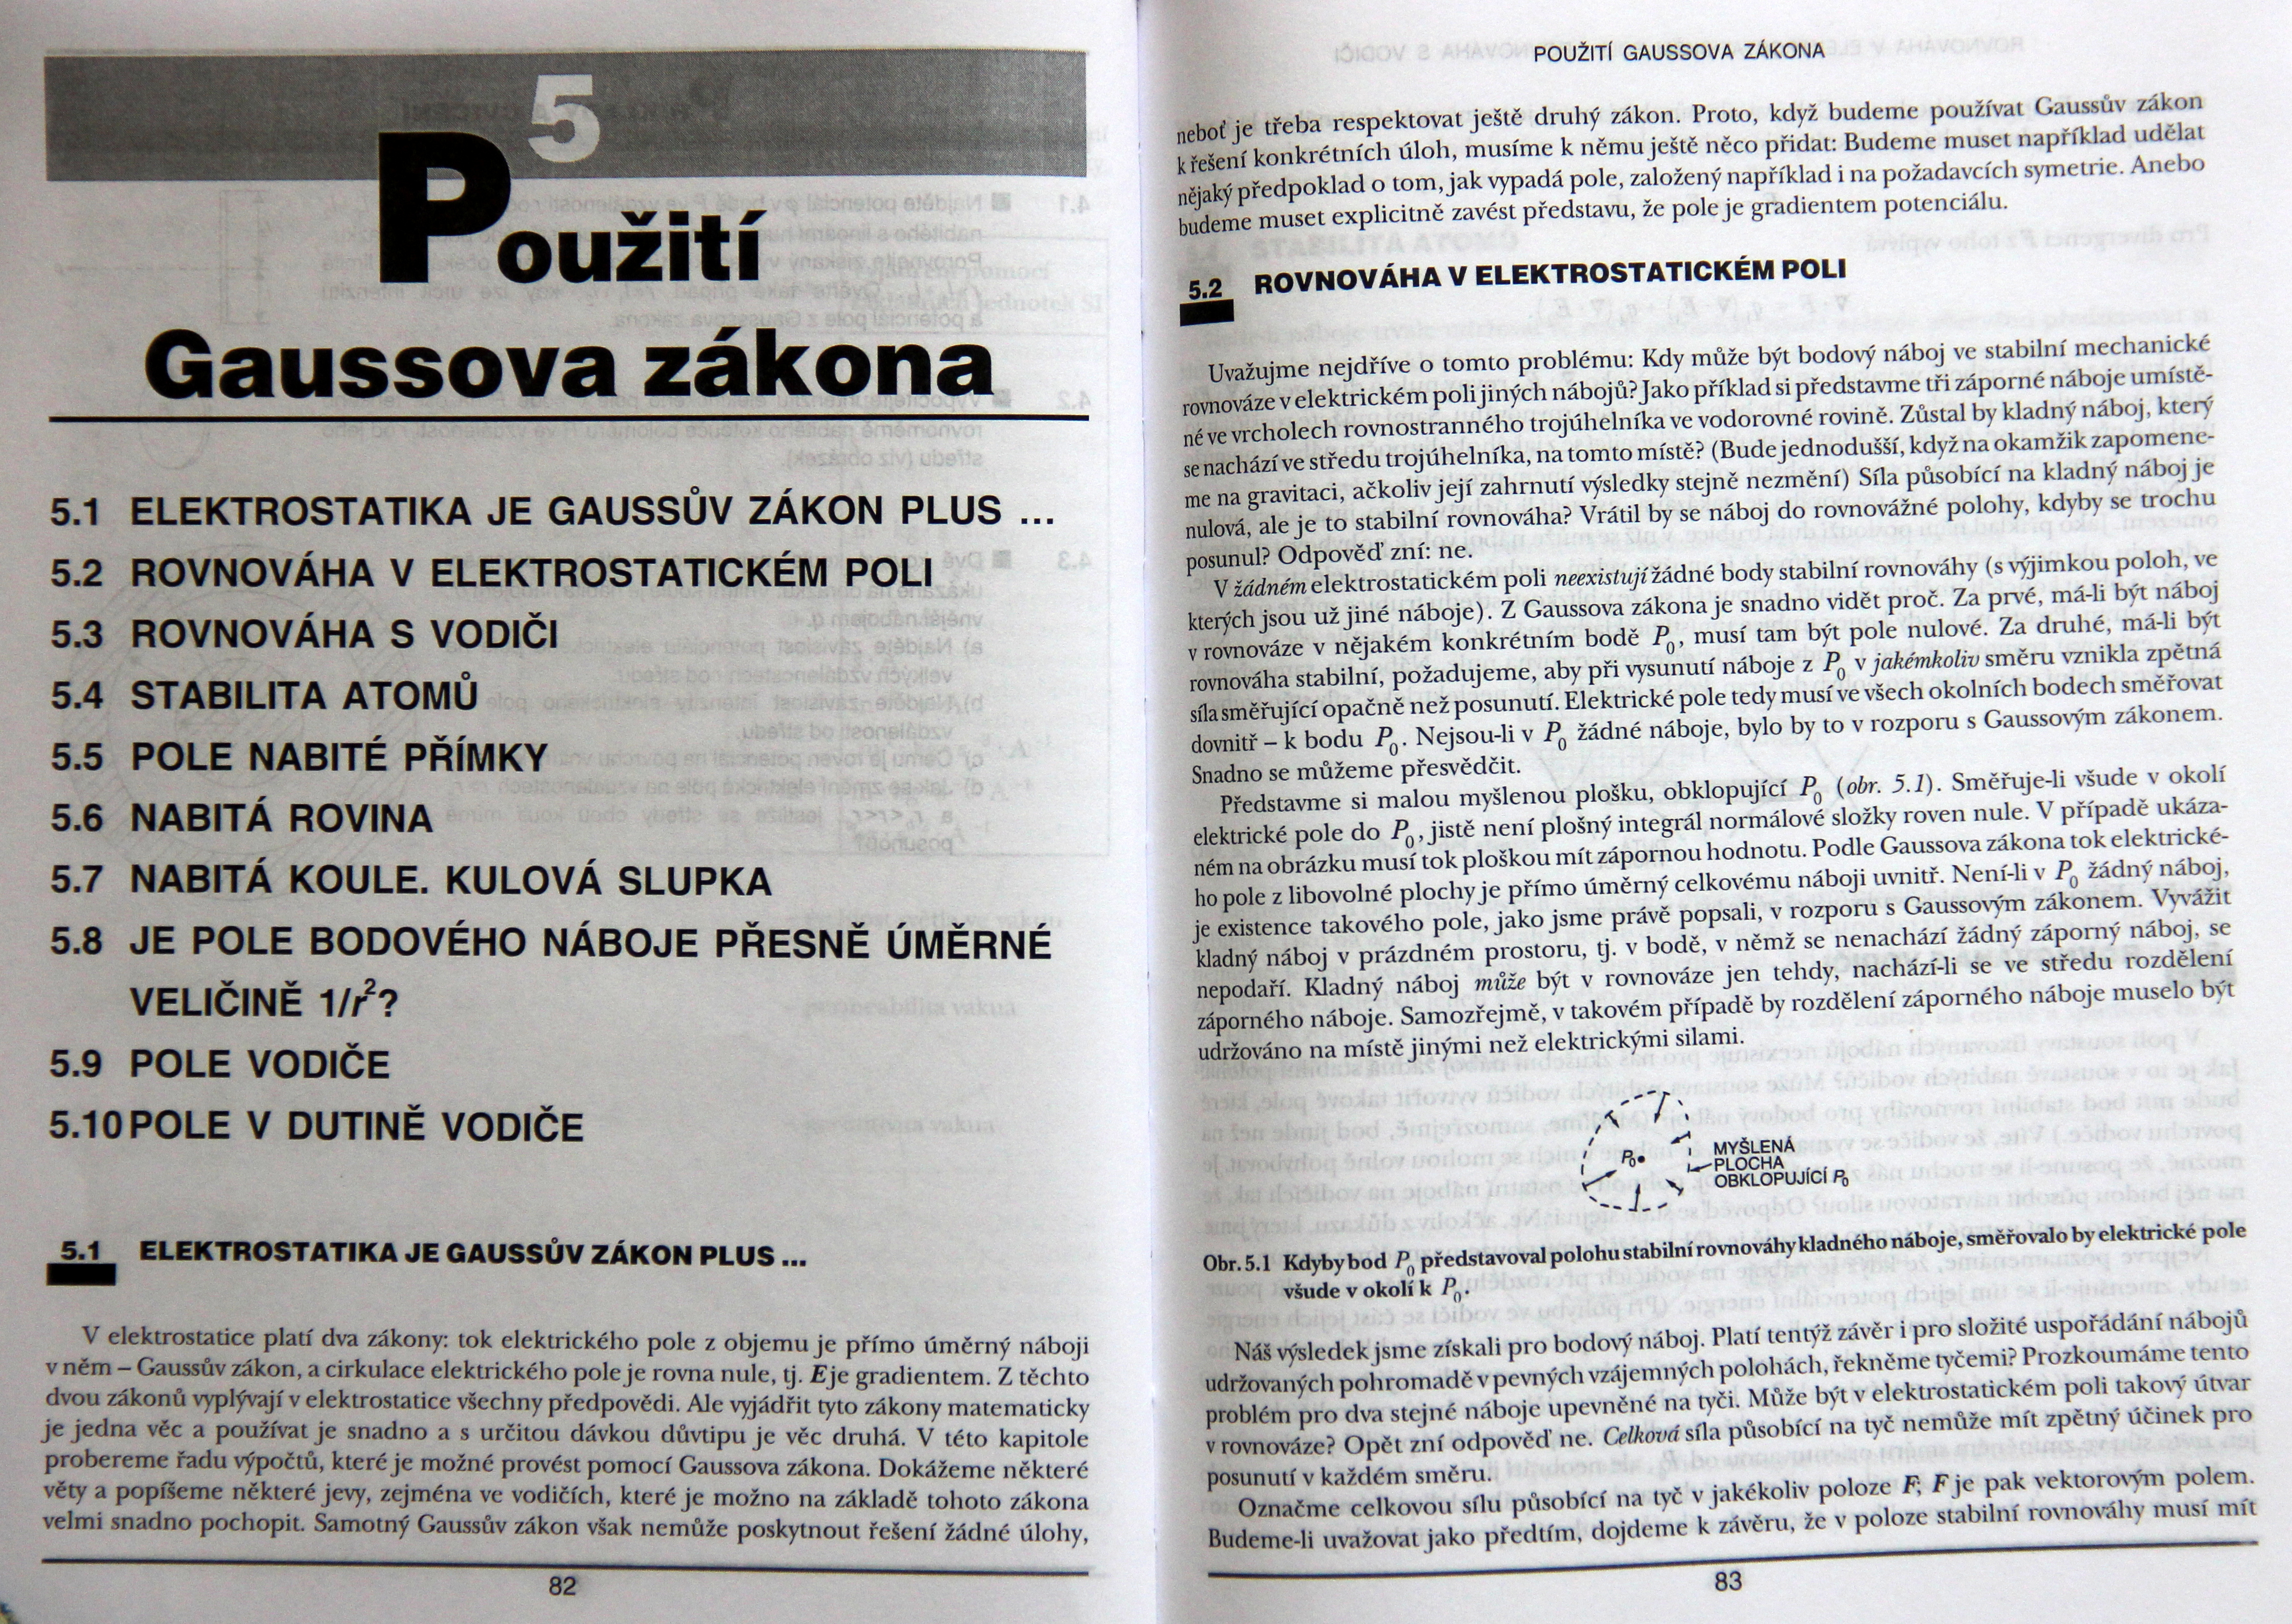
\includegraphics[width=0.6\linewidth]{fey_elstat_gauss01.jpg}
        \caption{Kdyby bod \(R\) představoval polohu stabilní rovnováhy kladného náboje, směřovalo by   
                 elektrické pole všude v okolí k \(P_0\).}
        \label{fyz:fig_fey_elstat_gauss01}
      \end{wrapfigure} 
      
      Označme celkovou sílu působící na tyč v jakékoliv poloze \(\vec{F}\); \(\vec{F}\) je pak vektorovým	
      polem. Budeme-li uvažovat jako předtím, dojdeme k závěru, že v poloze stabilní rovnováhy musí mít
      divergence \(\vec{F}\) zápornou hodnotu. Celková síla působící na tyč je rovna prvnímu náboji krát pole 
      v jeho poloze, plus druhý náboj krát pole v jeho poloze: 
      \begin{equation}\label{fyz:eq_fey_elstat_gauss01}
       \vec{F}=q_1\vec{E_1} + q_2\vec{E_2}. 
      \end{equation}
      Pro divergenci \(F\) z toho vyplývá \[\ndiver{F}=q_1(\ndiver{E_1}) + q_2(\ndiver{E_2}).\] Je-li každý z 
      těchto nábojů ve vakuu, jsou V \(q_1(\ndiver{E_1})\), stejně jako \(q_2(\ndiver{E_2})\) rovny nule a 
      divergence \(\ndiver{F}\) je také rovna nule - není tedy záporná, jak by bylo žádoucí pro rovnováhu. 
      Sami můžete rozšířit tuto úvahu a přesvědčit se, že vůbec žádný pevný útvar skládající se z jakéhokoliv 
      počtu nábojů nemůže mít v elektrostatickém poli polohu stabilní rovnováhy ve volném prostoru.
      
      Nedokázali jsme však, že rovnováha je zakázána, existují-li úchyty nebo jiná mechanická omezení. Jako 
      příklad nám poslouží dutá trubice, v níž se může náboj volně pohybovat dopředu a dozadu, ale ne do 
      stran. V tomto případě je možno velmi snadno navrhnout elektrické pole, které na obou koncích směřuje 
      dovnitř, připustí-li se, že v blízkosti středu trubice může směřovat ven do stran. Prostě na každý 
      konec trubice umístíme kladné náboje, jak ukazuje obr. \ref{fyz:fig_fey_elstat_gauss02}. Nyní může 
      existovat rovnovážný bod i tehdy, když je divergence rovna nule. Náboj by, samozřejmě, nebyl ve 
      stabilní rovnováze pro pohyb do stran, kdyby nepůsobily „neelektrické“ síly stěn trubice. 
      
      \begin{figure}[ht!] % \ref{fyz:fig_fey_elstat_gauss02}
        \centering
        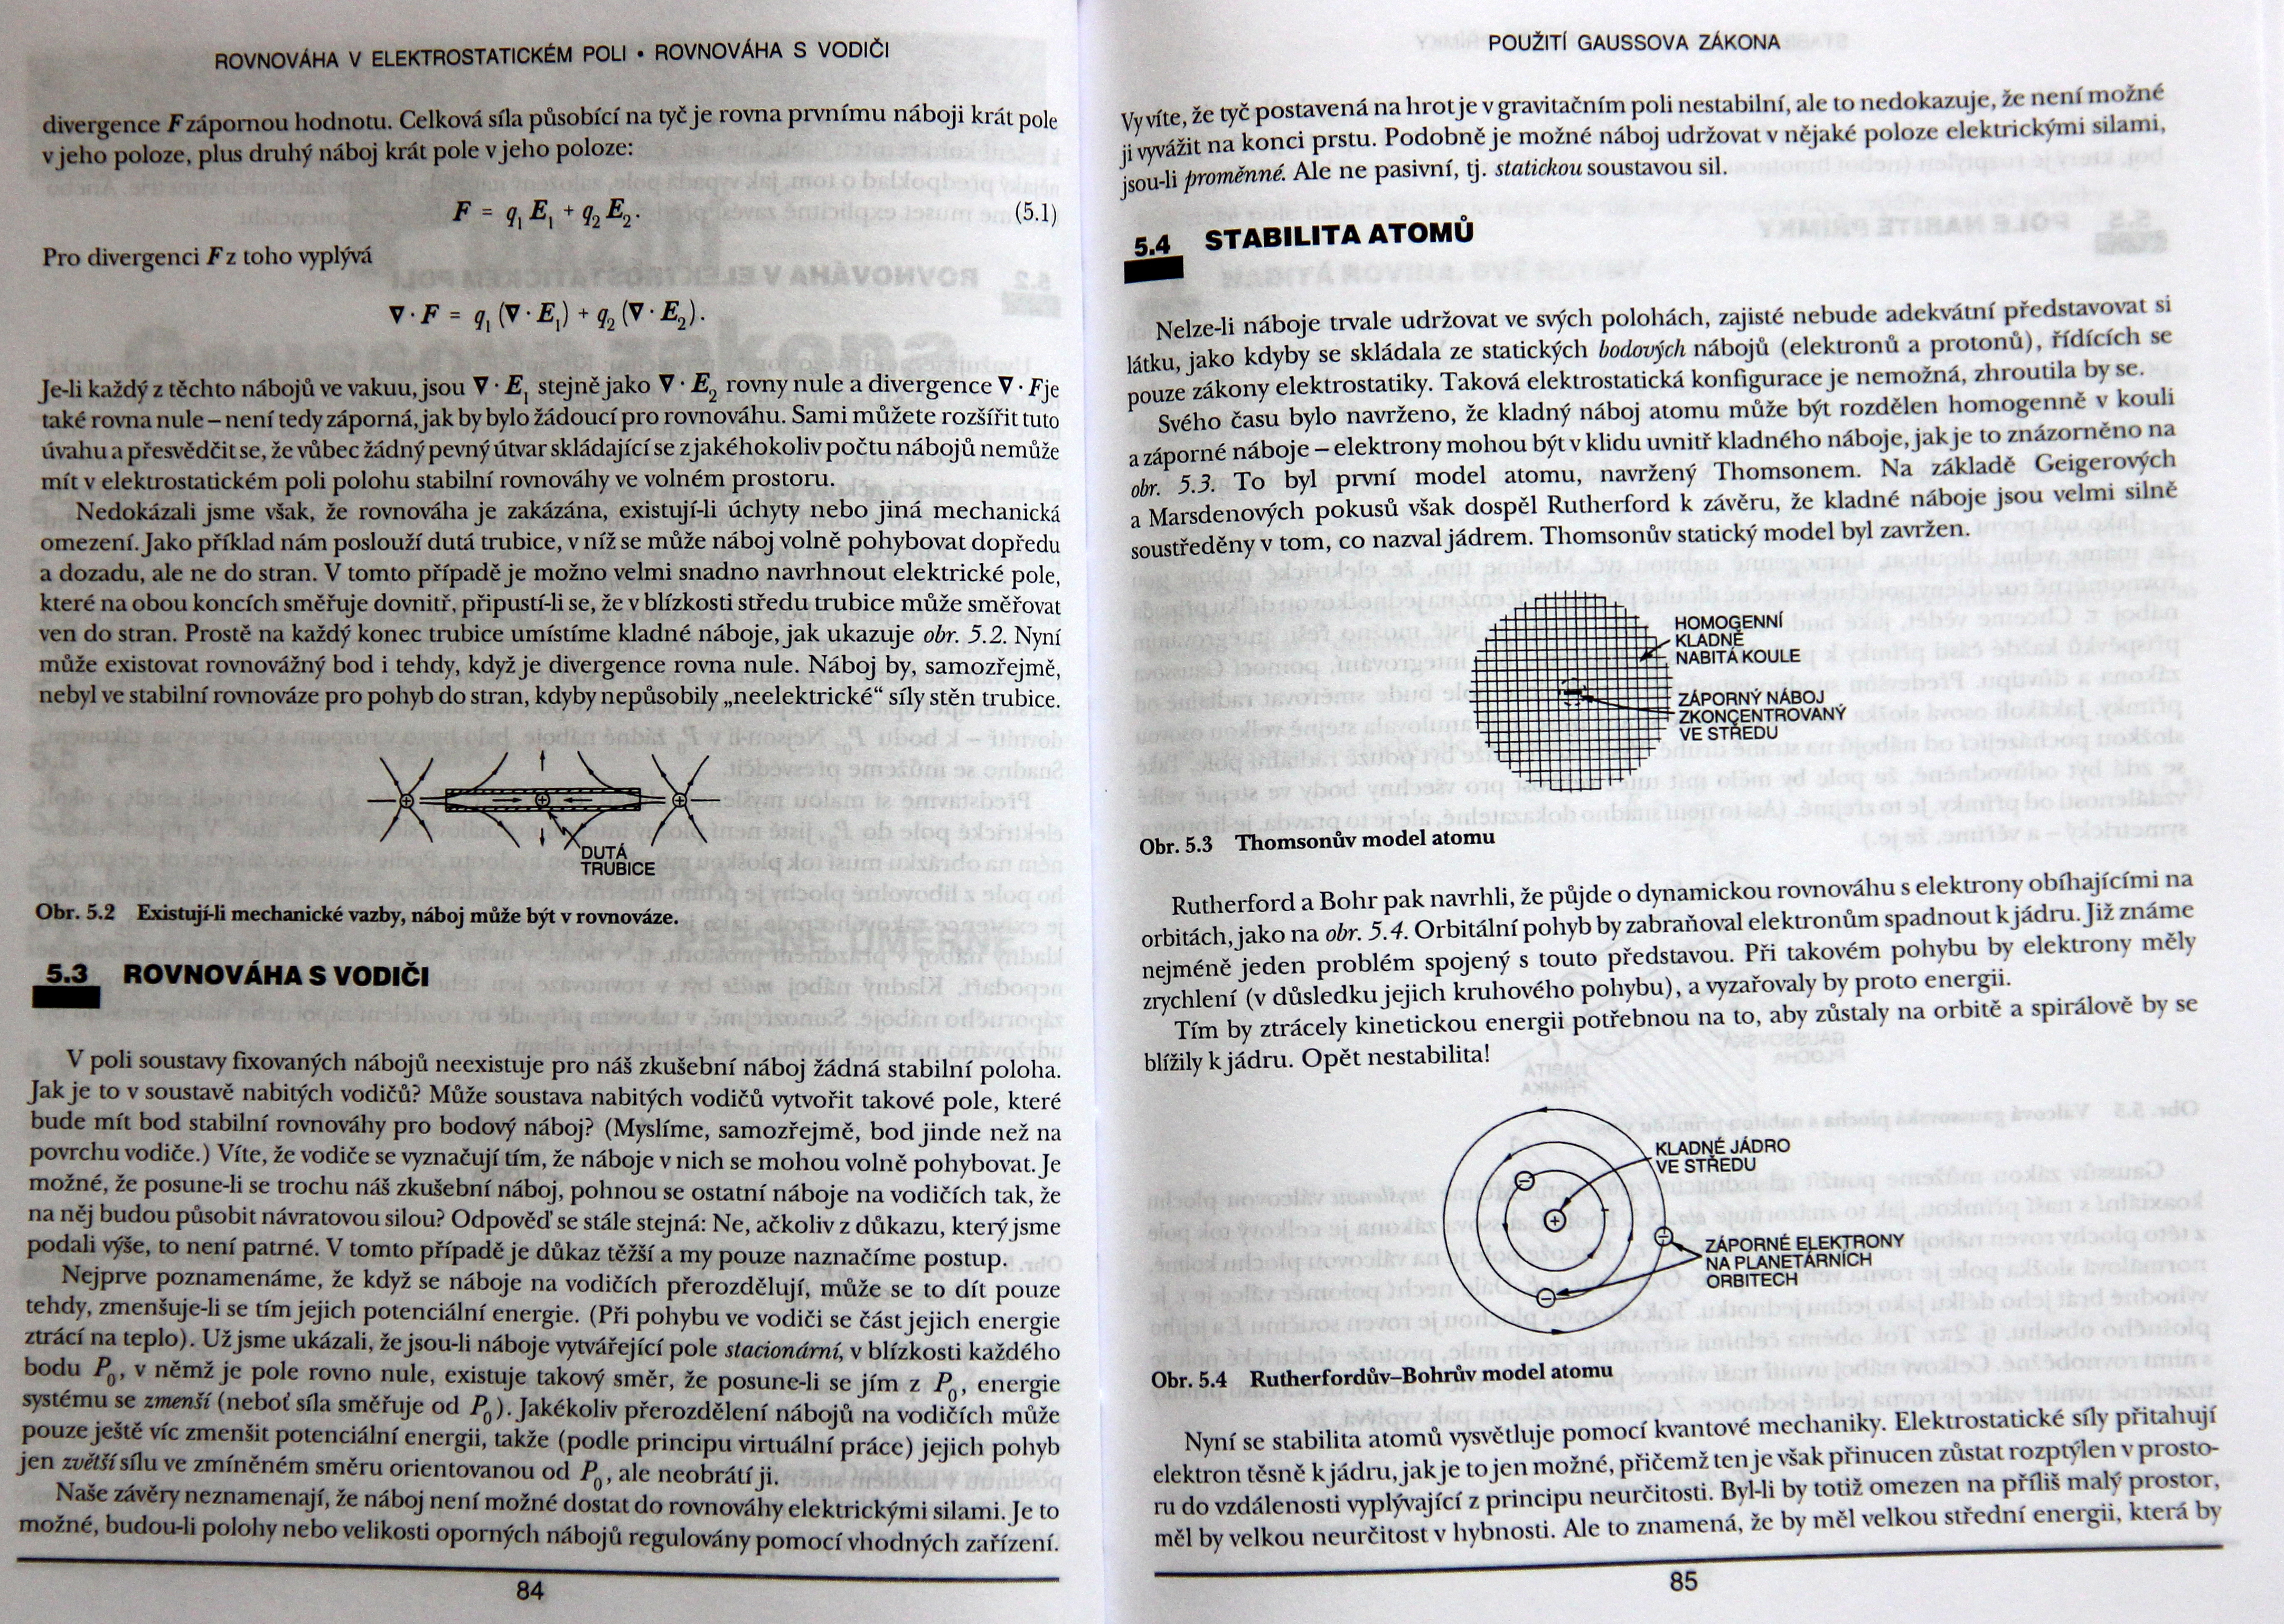
\includegraphics[width=0.6\linewidth]{fey_elstat_gauss02.jpg}
        \caption{Existují-li mechanické vazby, náboj může být v rovnováze.}
        \label{fyz:fig_fey_elstat_gauss02}
      \end{figure}      
      
    \subsection{Rovnováha s vodiči}
      V poli soustavy fixovaných nábojů neexistuje pro náš zkušební náboj žádná stabilní poloha. Jak je to v 
      soustavě nabitých vodičů? Může soustava nabitých vodičů vytvořit takové pole, které bude mít bod 
      stabilní rovnováhy pro bodový náboj? (Myslíme, samozřejmě, bod jinde než na povrchu vodiče.) Víte, že 
      vodiče se vyznačují tím, že náboje v nich se mohou volně pohybovat. Je možné, že posune-li se trochu 
      náš zkušební náboj, pohnou se ostatní náboje na vodičích tak, že na něj budou působit návratovou silou? 
      Odpověď se stále stejná: Ne, ačkoliv z důkazu, který jsme podali výše, to není patrné. V tomto případě 
      je důkaz těžší a my pouze naznačíme postup.
      
      \emph{Nejprve poznamenáme, že když se náboje na vodičích přerozdělují, může se to dít pouze tehdy, 
      zmenšuje-li se tím jejich potenciální energie}. (Při pohybu ve vodiči se část jejich energie ztrácí na 
      teplo). Už jsme ukázali, že jsou-li náboje vytvářející pole \emph{stacionární}, v blízkosti každého 
      bodu \(P_0\), v němž je pole rovno nule, existuje takový směr, že posune-li se jím z \(P_0\), energie 
      systému se zmenší (neboť síla směřuje od \(P_0\)). Jakékoliv přerozdělení nábojů na vodičích může pouze 
      ještě víc zmenšit potenciální energii, takže (podle principu virtuální práce) jejich pohyb jen zvětší 
      sílu ve zmíněném směru orientovanou od \(P_0\), ale neobrátí ji.
      
      Naše závěry neznamenají, že náboj není možné dostat do rovnováhy elektrickými silami. Je to možné, 
      budou-li polohy nebo velikosti opěrných nábojů regulovány pomocí vhodných zařízení. Vy víte, že tyč 
      postavená na hrot je v gravitačním poli nestabilní, ale to nedokazuje, že není možné ji vyvážit na 
      konci prstu. Podobně je možné náboj udržovat v nějaké poloze elektrickými silami, jsou-li 
      \emph{proměnné}. Ale ne pasivní, tj. \emph{statickou} soustavou sil.
    
    \subsection{Stabilita atomů}
      Nelze-li náboje trvale udržovat ve svých polohách, zajisté nebude adekvátní představovat si látku, jako 
      kdyby se skládala ze statických bodových nábojů (elektronů a protonů), řídících se pouze zákony 
      elektrostatiky. Taková elektrostatická konfigurace je nemožná, zhroutila by se.
      
      Svého času bylo navrženo, že kladný náboj atomu může být rozdělen homogenně v kouli a záporné náboje — 
      elektrony mohou být v klidu uvnitř kladného náboje, jak je to znázorněno na obr. 
      \ref{fyz:fig_fey_elstat_gauss03}. To byl první model atomu, navržený Thomsonem. Na základě Geigerových 
      a Marsdenových pokusů však dospěl Rutherford k závěru, že kladné náboje jsou velmi silně soustředěny v 
      tom, co nazval jádrem. Thomsonův statický model 
      byl zavržen.
      \begin{figure}[ht!] % \ref{fyz:fig_fey_elstat_gauss03}
        \centering
        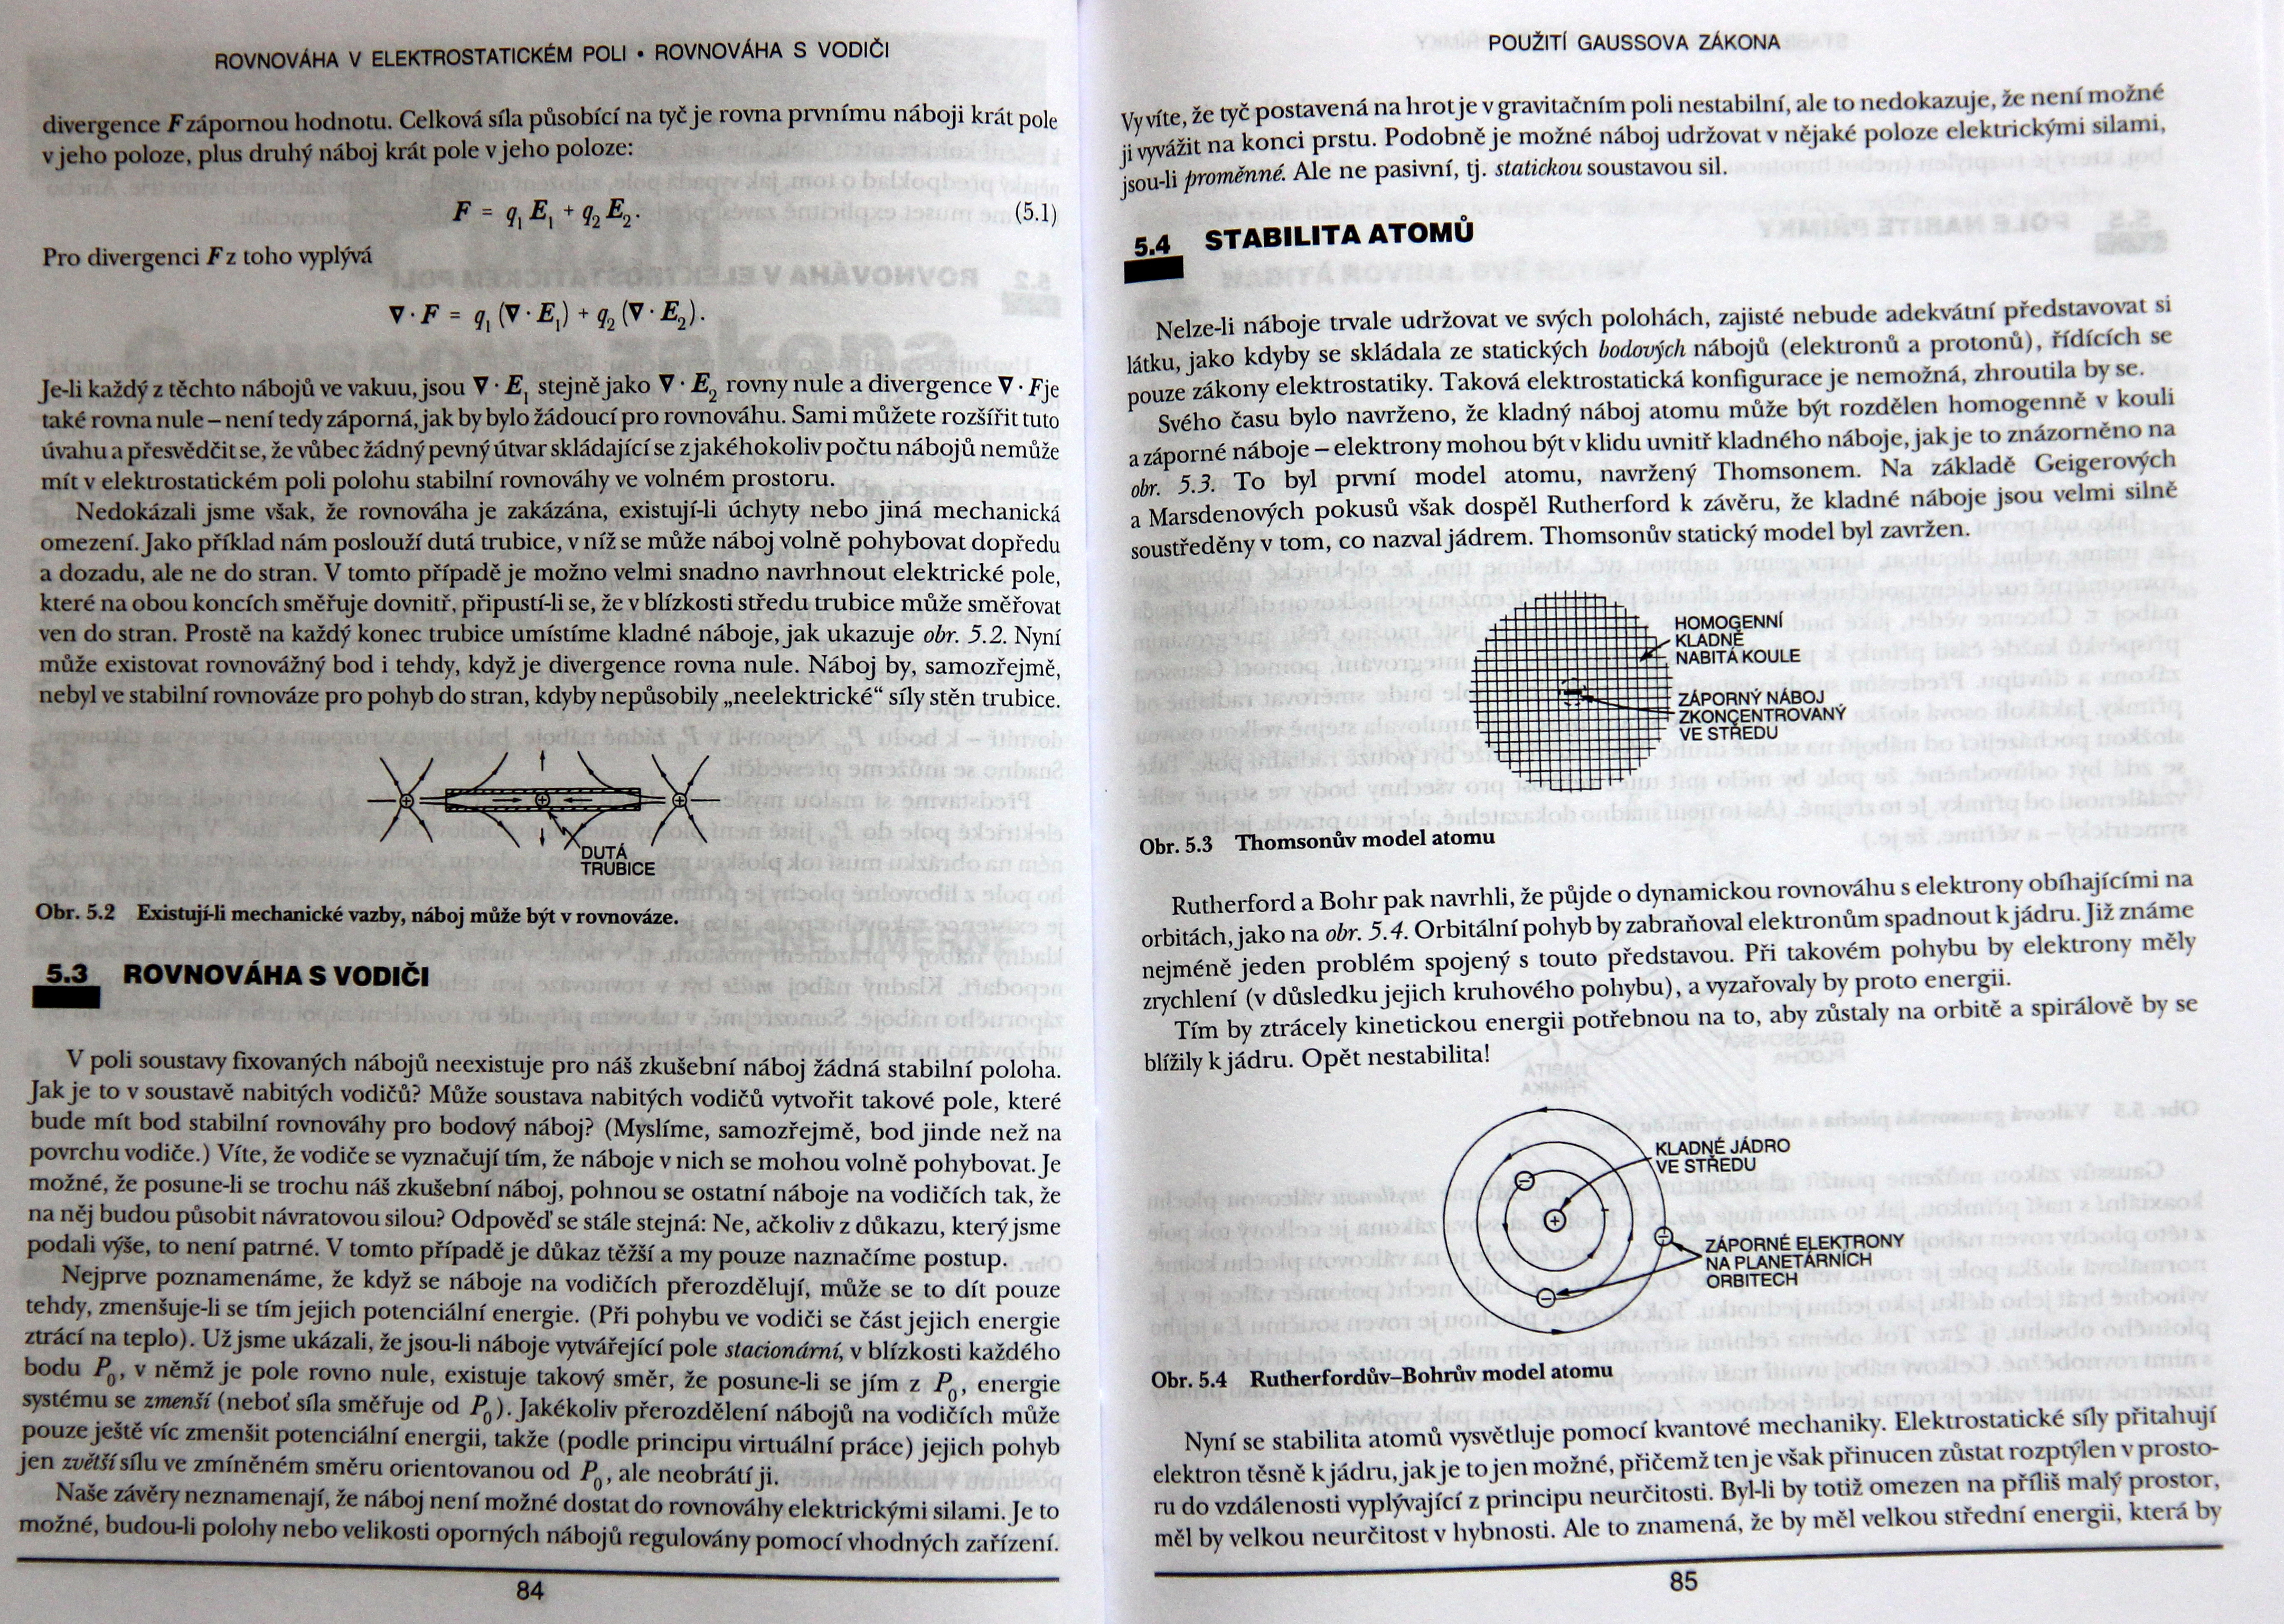
\includegraphics[width=0.6\linewidth]{fey_elstat_gauss03.jpg}
        \caption{Thomsonův model atomu}
        \label{fyz:fig_fey_elstat_gauss03}
      \end{figure}
      
      Rutherford a Bohr pak navrhli, že půjde o dynamickou rovnováhu s elektrony obíhajícími na orbitách, 
      jako na obr. \ref{fyz:fig_fey_elstat_gauss04}. Orbitální pohyb by zabraňoval elektronům spadnout k 
      jádru. Již známe nejméně jeden problém spojený s touto představou. Při takovém pohybu by elektrony měly 
      zrychlení (v důsledku jejich kruhového pohybu), a vyzařovaly by proto energii.
      
      Tím by ztrácely kinetickou energii potřebnou na to, aby zůstaly na orbitě a spirálově by se blížily k 
      jádru. Opět nestabilita!
      \begin{figure}[ht!] % \ref{fyz:fig_fey_elstat_gauss04}
        \centering
        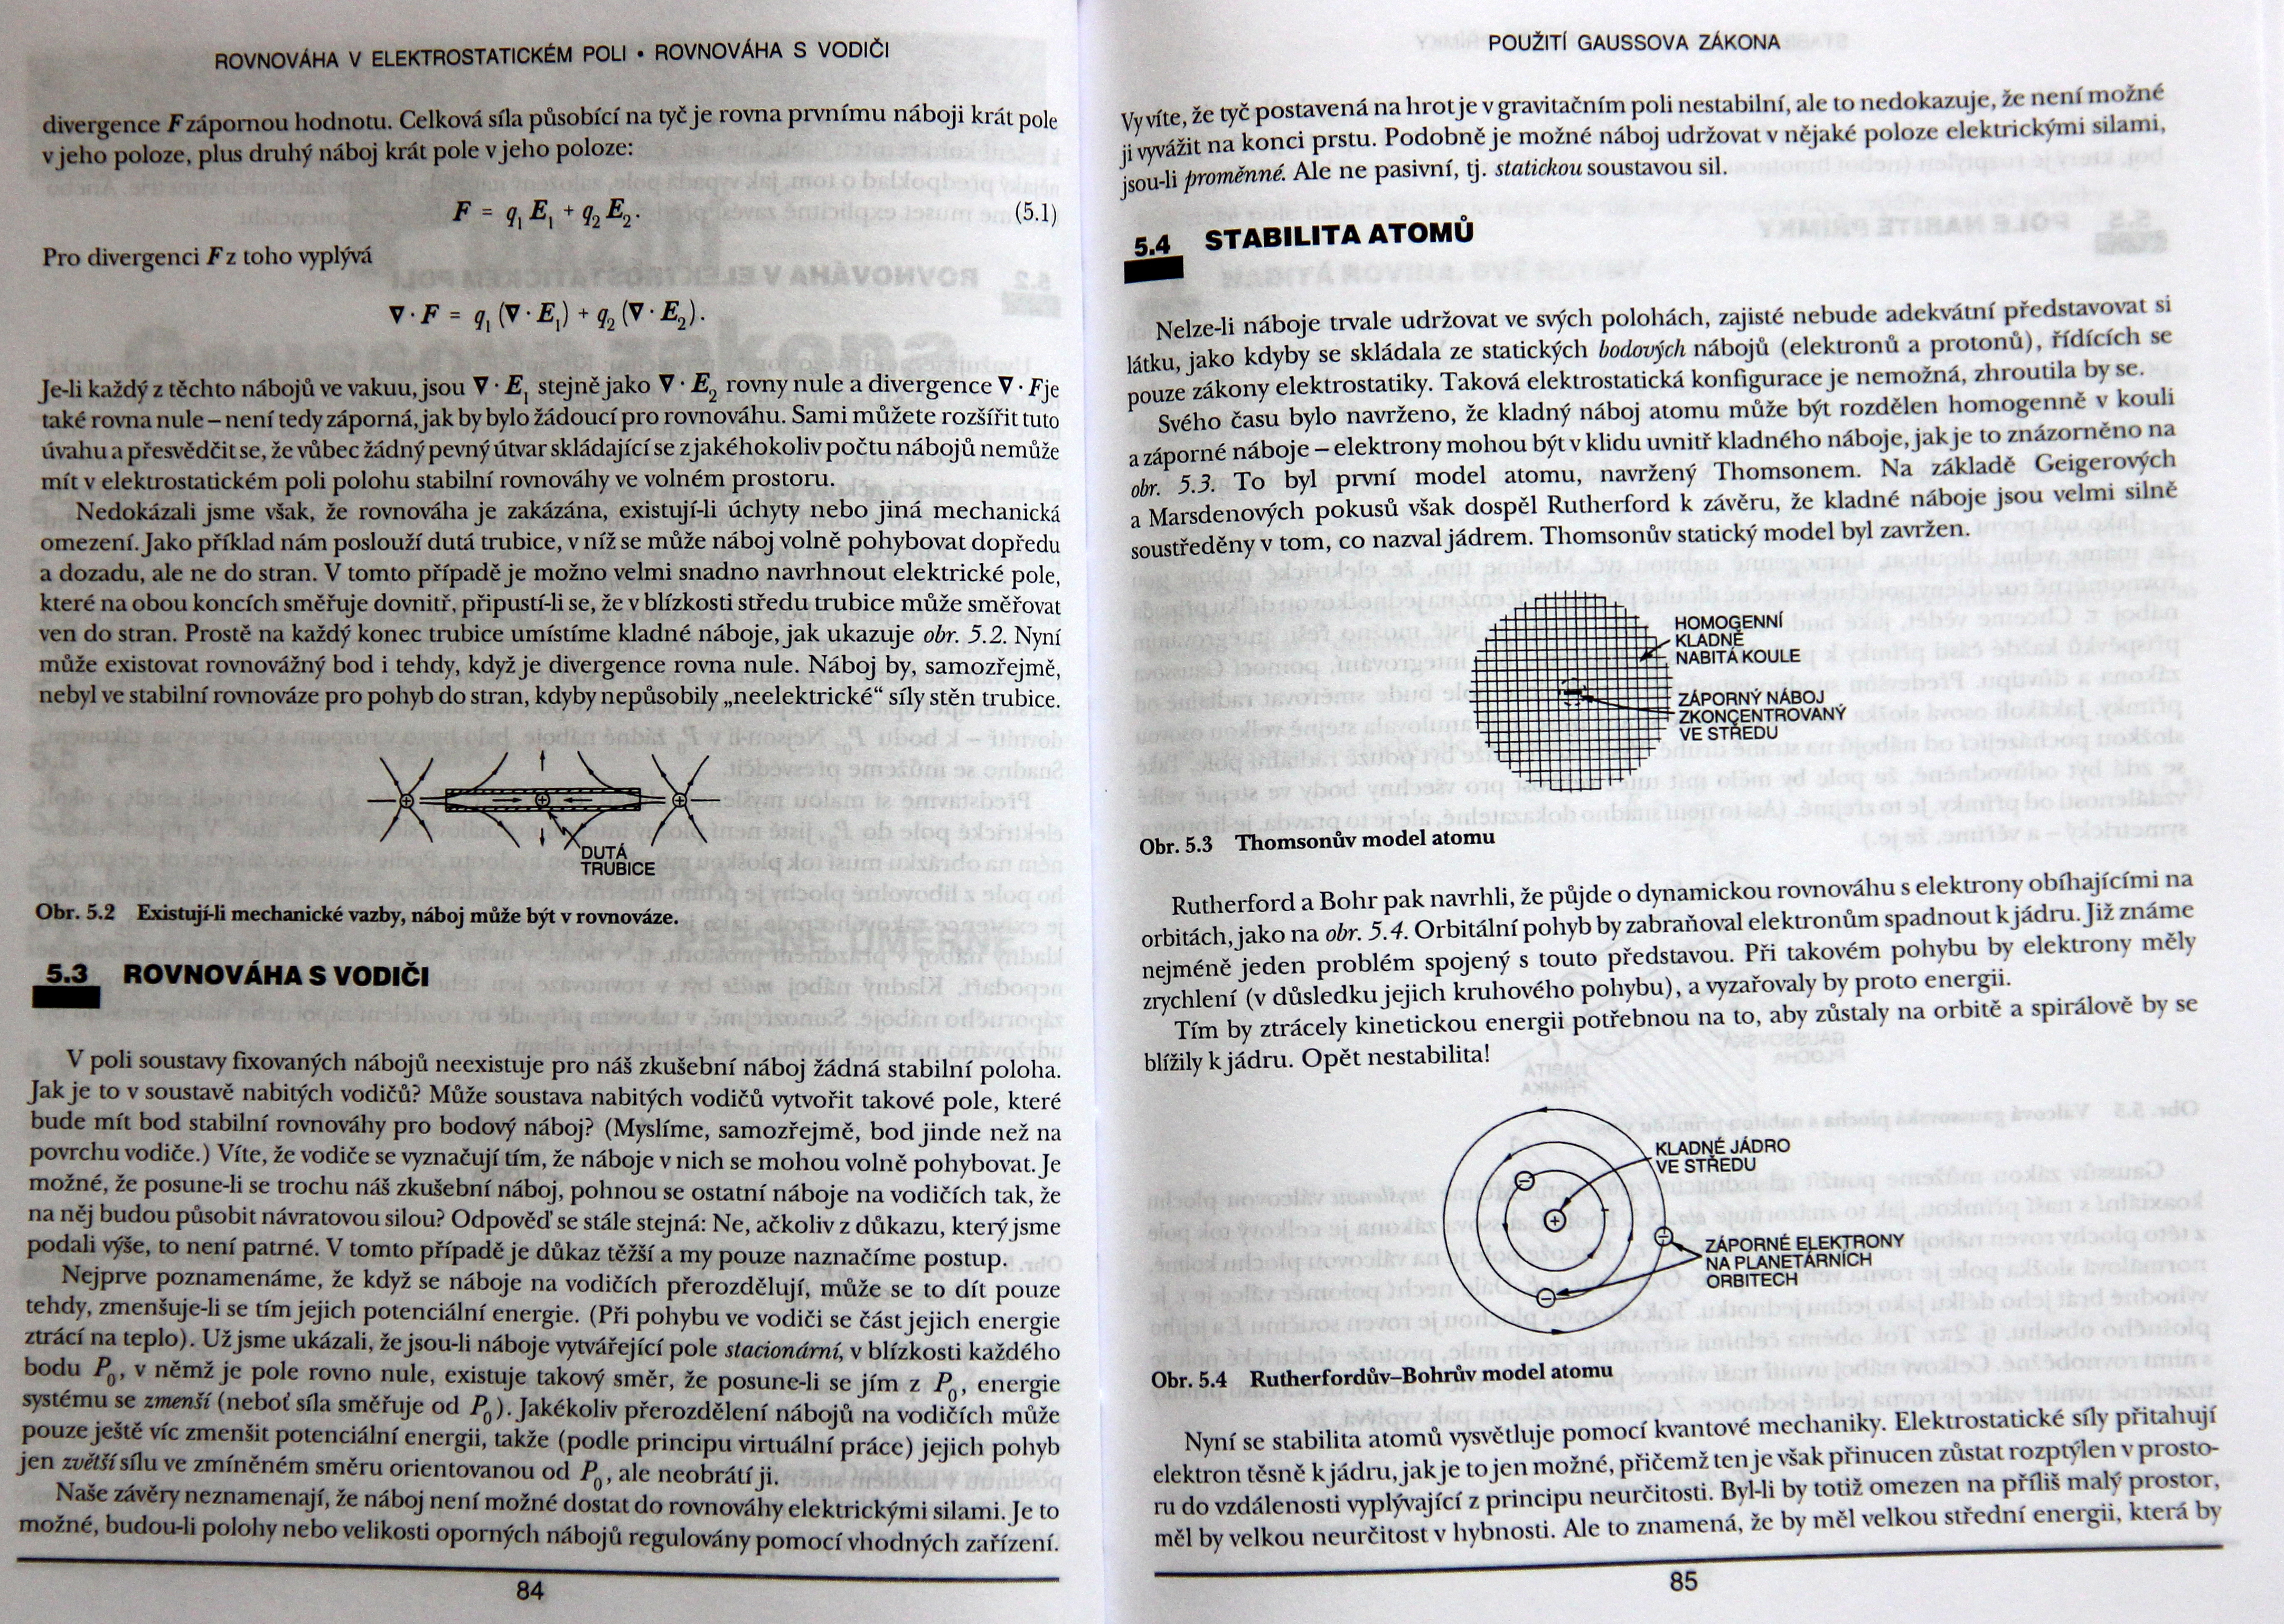
\includegraphics[width=0.6\linewidth]{fey_elstat_gauss04.jpg}
        \caption{Rutherfordův-Bohrův model atomu}
        \label{fyz:fig_fey_elstat_gauss04}
      \end{figure}      
      
      Nyní se stabilita atomů vysvětluje pomocí kvantové mechaniky. Elektrostatické síly přitahují elektron 
      těsně k jádru, jak je to jen možné, přičemž ten je však přinucen zůstat rozptýlen v prostoru do 
      vzdálenosti vyplývající z principu neurčitosti. Byl-li by totiž omezen na příliš malý prostor, měl by 
      velkou neurčitost v hybnosti. Ale to znamená, že by měl velkou střední energii, která by mu umožňovala 
      vymanit se z elektrické přitažlivosti jádra. Konečným výsledkem je taková elektrická rovnováha, která 
      se ani příliš neliší od Thomsonovy představy - pouze je to záporný náboj, který je rozptýlen (neboť 
      hmotnost elektronu je mnohokrát menší než hmotnost protonu).
    
    \subsection{Pole nabité přímky}
      Gaussův zákon je možno použít na řešení mnoha úloh o elektrostatickém poli vyznačujících se speciální 
      symetrií - obvykle kulovou, válcovou nebo rovinnou. Ve zbývající částí této kapitoly použijeme Gaussův 
      zákon v několika takových úlohách. Snadnost, s jakou lze tyto úlohy takto řešit, může vést ke klamnému 
      dojmu, že jde o velmi účinnou metodu umožňující postupovat tak i v mnoha dalších úlohách. Naneštěstí 
      tomu tak není. Seznam úloh, které lze pomocí Gaussova zákona snadno řešit, bude brzy vyčerpán. V 
      dalších kapitolách vypracujeme účinnější metody ke zkoumání elektrostatických polí.
      
      Jako náš první příklad budeme uvažovat soustavu s válcovou souměrností. Předpokládejme, že máme velmi 
      dlouhou, homogenně nabitou tyč. Myslíme tím, že elektrické náboje jsou rovnoměrně rozděleny podél 
      nekonečně dlouhé přímky, přičemž na jednotkovou délku připadá náboj \(\tau\). Chceme vědět, jaké bude 
      elektrické pole. Úlohu je jistě možno řešit integrováním příspěvků každé části přímky k poli. My to 
      však dokážeme bez integrování, pomocí Gaussova zákona a důvtipu. Především snadno vytušíme, že 
      elektrické pole bude směřovat radiálně od přímky. Jakákoli osová složka nábojů na jedné straně by se 
      totiž anulovala stejně velkou osovou složkou pocházející od nábojů na straně druhé. Výsledkem může být 
      pouze radiální pole. Také se zdá být odůvodněné, že pole by mělo mít tutéž velikost pro všechny body ve 
      stejně velké vzdálenosti od přímky. Je to zřejmé. (Asi to není snadno dokazatelné, ale je to pravda, 
      je-li prostor symetrický - a věříme, že je.)
      
      \begin{figure}[ht!] % \ref{fyz:fig_fey_elstat_gauss05}
        \centering
        \includegraphics[width=0.6\linewidth]{fey_elstat_gauss05.jpg}
        \caption{Válcová gaussovská plocha s nabitou přímkou v ose}
        \label{fyz:fig_fey_elstat_gauss05}
      \end{figure}  
      
      Gaussův zákon můžeme použít následujícím způsobem. Mějme myšlenou válcovou plochu koaxiální s naší 
      přímkou, jak to znázorňuje obr. \ref{fyz:fig_fey_elstat_gauss05}. Podle Gaussova zákona je celkový tok 
      pole z této plochy roven náboji uvnitř válce, dělenému \(\varepsilon_0\). Protože pole je na válcovou 
      plochu kolmé, normálová složka pole je rovna velikosti pole. Označíme ji \(E\). Dále nechť poloměr 
      válce je \(r\). Je výhodné brát jeho délku jako jednotkovou. Tok válcovou plochou je roven součinu 
      \(E\) a jejího plošného obsahu, tj. \(2\pi r\). Tok oběma čelními stěnami je roven nule, protože 
      elektrické pole je s nimi rovnoběžné. Celkový náboj uvnitř naší válcové plochy je přesně \(\tau\), 
      neboť délka části přímky uzavřené uvnitř válce je rovna jedné jednotce. Z Gaussova zákona pak vyplývá, 
      že
      \begin{equation}\label{fyz:eq_fey_elstat_gauss02}
        E\cdot2\pi r = \frac{\tau}{\varepsilon_0} \Rightarrow E = \frac{\tau}{2\pi\varepsilon_0 r}
      \end{equation}
      Elektrické pole nabité přímky je nepřímo úměrné \emph{první} mocnině vzdálenosti od přímky.
    
    \subsection{Nabitá rovina, dvě roviny}
      V dalším příkladě budeme počítat pole homogenně nabité roviny. Předpokládejme, že rovina se rozprostírá 
      do nekonečna a na její plošnou jednotku připadá náboj \(\sigma\). Teď provedeme další odhad. Důvody 
      souměrnosti nás totiž vedou k přesvědčení, že směr pole je všude kolmý na rovinu a že 
      \emph{neexistuje-li pole jiných nábojů}, musí být pole na obou stranách roviny stejné (co do 
      velikostí). Tentokrát zvolme jako naši gaussovskou plochu pravoúhlou krabičku, která protíná uvažovanou 
      rovinu (obr. \ref{fyz:fig_fey_elstat_gauss06}). Stěny krabičky rovnoběžné s rovinou budou mít stejný 
      plošný obsah \(S\). Pole je na tyto dvě stěny kolmé a se zbývajícími čtyřmi stěnami je rovnoběžné. 
      Celkový tok je roven \(E-\text{krát}\) plošnému obsahu první stěny plus \(E-\text{krát}\) plošný obsah 
      protilehlé stěny, přičemž zbývající čtyři stěny nepřispívají ničím. Celkový náboj uvnitř krabičky je 
      \(\sigma\cdot S\). Když jej uvedeme do vztahu s tokem stěnami krabice, dostaneme rovnost
      \begin{equation}\label{fyz:eq_fey_elstat_gauss03}
        E\cdot S + E\cdot S = \frac{\sigma\cdot S}{\varepsilon_0} \Rightarrow 
        E = \frac{\sigma}{2\varepsilon_0}.
      \end{equation}
      
      \begin{figure}[ht!] % \ref{fyz:fig_fey_elstat_gauss06}
        \centering
        \includegraphics[width=0.6\linewidth]{fey_elstat_gauss06.jpg}
        \caption{Elektrické pole v blízkosti homogenně nabité roviny je možno najít použitím Gaussova zákona 
                 na myšlenou krabici.}
        \label{fyz:fig_fey_elstat_gauss06}
      \end{figure}
      
      Tentýž výsledek jsme dostali už dříve integrováním po celé ploše. Gaussův zákon nám dává odpověď v 
      tomto příkladě o mnoho rychleji (ačkoli nemá takovou obecnou použitelnost jako dřívější metoda).
      
      Zdůrazňujeme, že tento výsledek se vztahuje pouze na pole vytvořené náboji rozmístěnými v rovině. 
      Nacházejí-li se někde v blízkostí ještě další náboje, bude celkové pole v okolí roviny rovno součtu 
      pole (\ref{fyz:eq_fey_elstat_gauss03}) a pole pocházejícího od těchto nábojů.
      
      Úloha se dvěma rovnoběžnými rovinami se stejnými plošnými hustotami nábojů, které mají opačná znaménka 
      \(+\sigma\) a \(-\sigma\), je také jednoduchá, předpokládáme-li opět, že vnější svět je zcela souměrný. 
      Superpozicí obou řešení pro jednotlivé roviny nebo sestrojením gaussovské krabice, která by proťala obě 
      roviny, je možno jednoduše ozřejmit, že na vnější straně rovin je pole rovno nule (obr. 
      \ref{fyz:fig_fey_elstat_gauss07}a). Kdybychom uvažovali krabici, která protíná jen jednu z rovin částí 
      b, c obrázku), mohli bychom se přesvědčit, že pole mezi deskami musí být dvakrát větší než v případě 
      jedni desky. Podle Gaussova zákona by pak platilo, že
      \begin{equation}\label{fyz:eq_fey_elstat_gauss04}
        E_1 + E_2 = \frac{\sigma}{\varepsilon_0}
      \end{equation}
      kde \(E_1\) a \(E_1\) jsou pole na každé straně roviny směřující od ní.
      \begin{figure}[ht!] % \ref{fyz:fig_fey_elstat_gauss07}
        \centering
        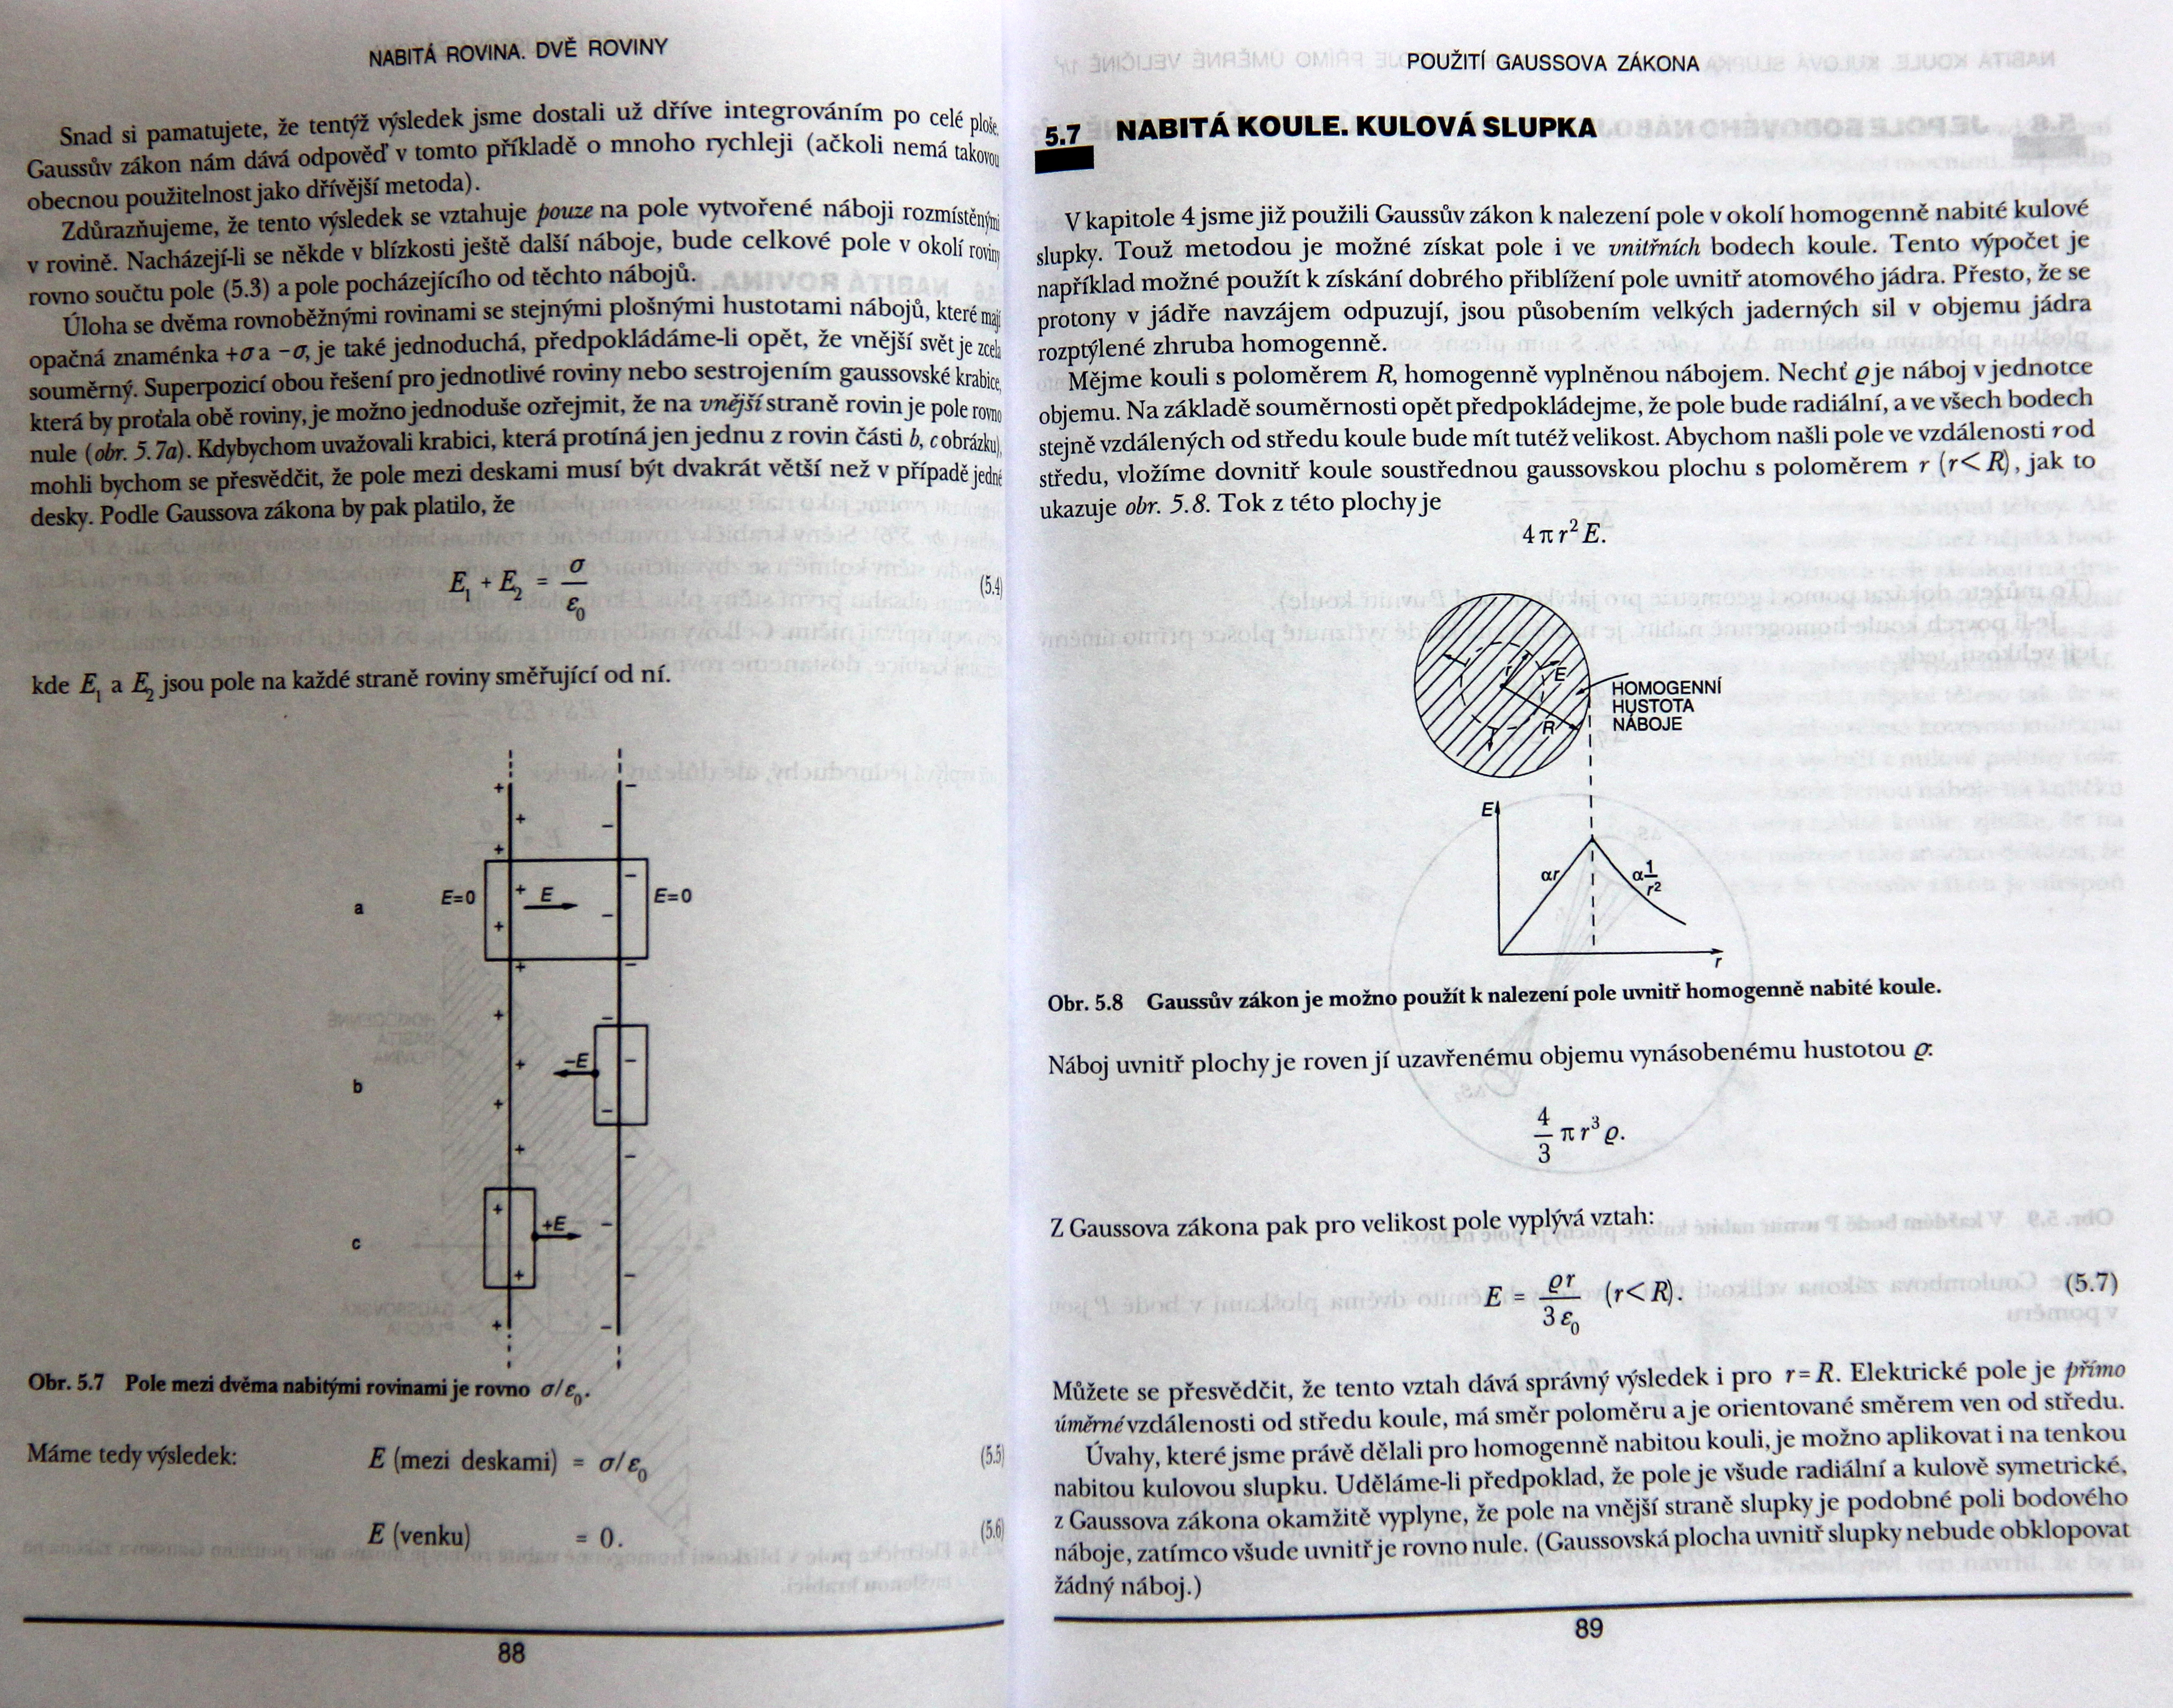
\includegraphics[width=0.6\linewidth]{fey_elstat_gauss07.jpg}
        \caption{Pole mezi dvěma nabitými rovinami je rovno \(\frac{\sigma}{\varepsilon_0}\)}
        \label{fyz:fig_fey_elstat_gauss07}
      \end{figure}
      Máme tedy výsledek
      \begin{align}
        E (\text{mezi deskami}) &= \frac{\sigma}{\varepsilon_0} \\
        E (\text{venku})        &= 0  
      \end{align}
      
    \subsection{Nabitá koule, kulová slupka}
      V kapitole \ref{fyz:chap_fey_ponako} jsme již použili Gaussův zákon k nalezení pole v okolí homogenně 
      nabité kulové slupky. Touž metodou je možné získat pole i ve vnitřních bodech koule. Tento výpočet je 
      například možné použít k získání dobrého přiblížení pole uvnitř atomového jádra. Přesto, že se protony 
      v jádře navzájem odpuzují, jsou působením velkých jaderných sil v objemu jádra rozptýlené zhruba 
      homogenně.
      
      Mějme kouli s poloměrem \(R\), homogenně vyplněnou nábojem. Nechť \(\varrho\) je náboj v jednotce 
      objemu. Na základě souměrnosti opět předpokládejme, že pole bude radiální, a ve všech bodech stejně 
      vzdálených od středu koule bude mít tutéž velikost. Abychom našli pole ve vzdálenosti \(r\) od středu, 
      vložíme dovnitř koule soustřednou gaussovskou plochu s poloměrem \(r\) \((r< R)\), jak to ukazuje obr. 
      \ref{fyz:fig_fey_elstat_gauss08}. Tok z této plochy je \[4\pi r^2E.\]
      \begin{figure}[ht!] % \ref{fyz:fig_fey_elstat_gauss08}
        \centering
        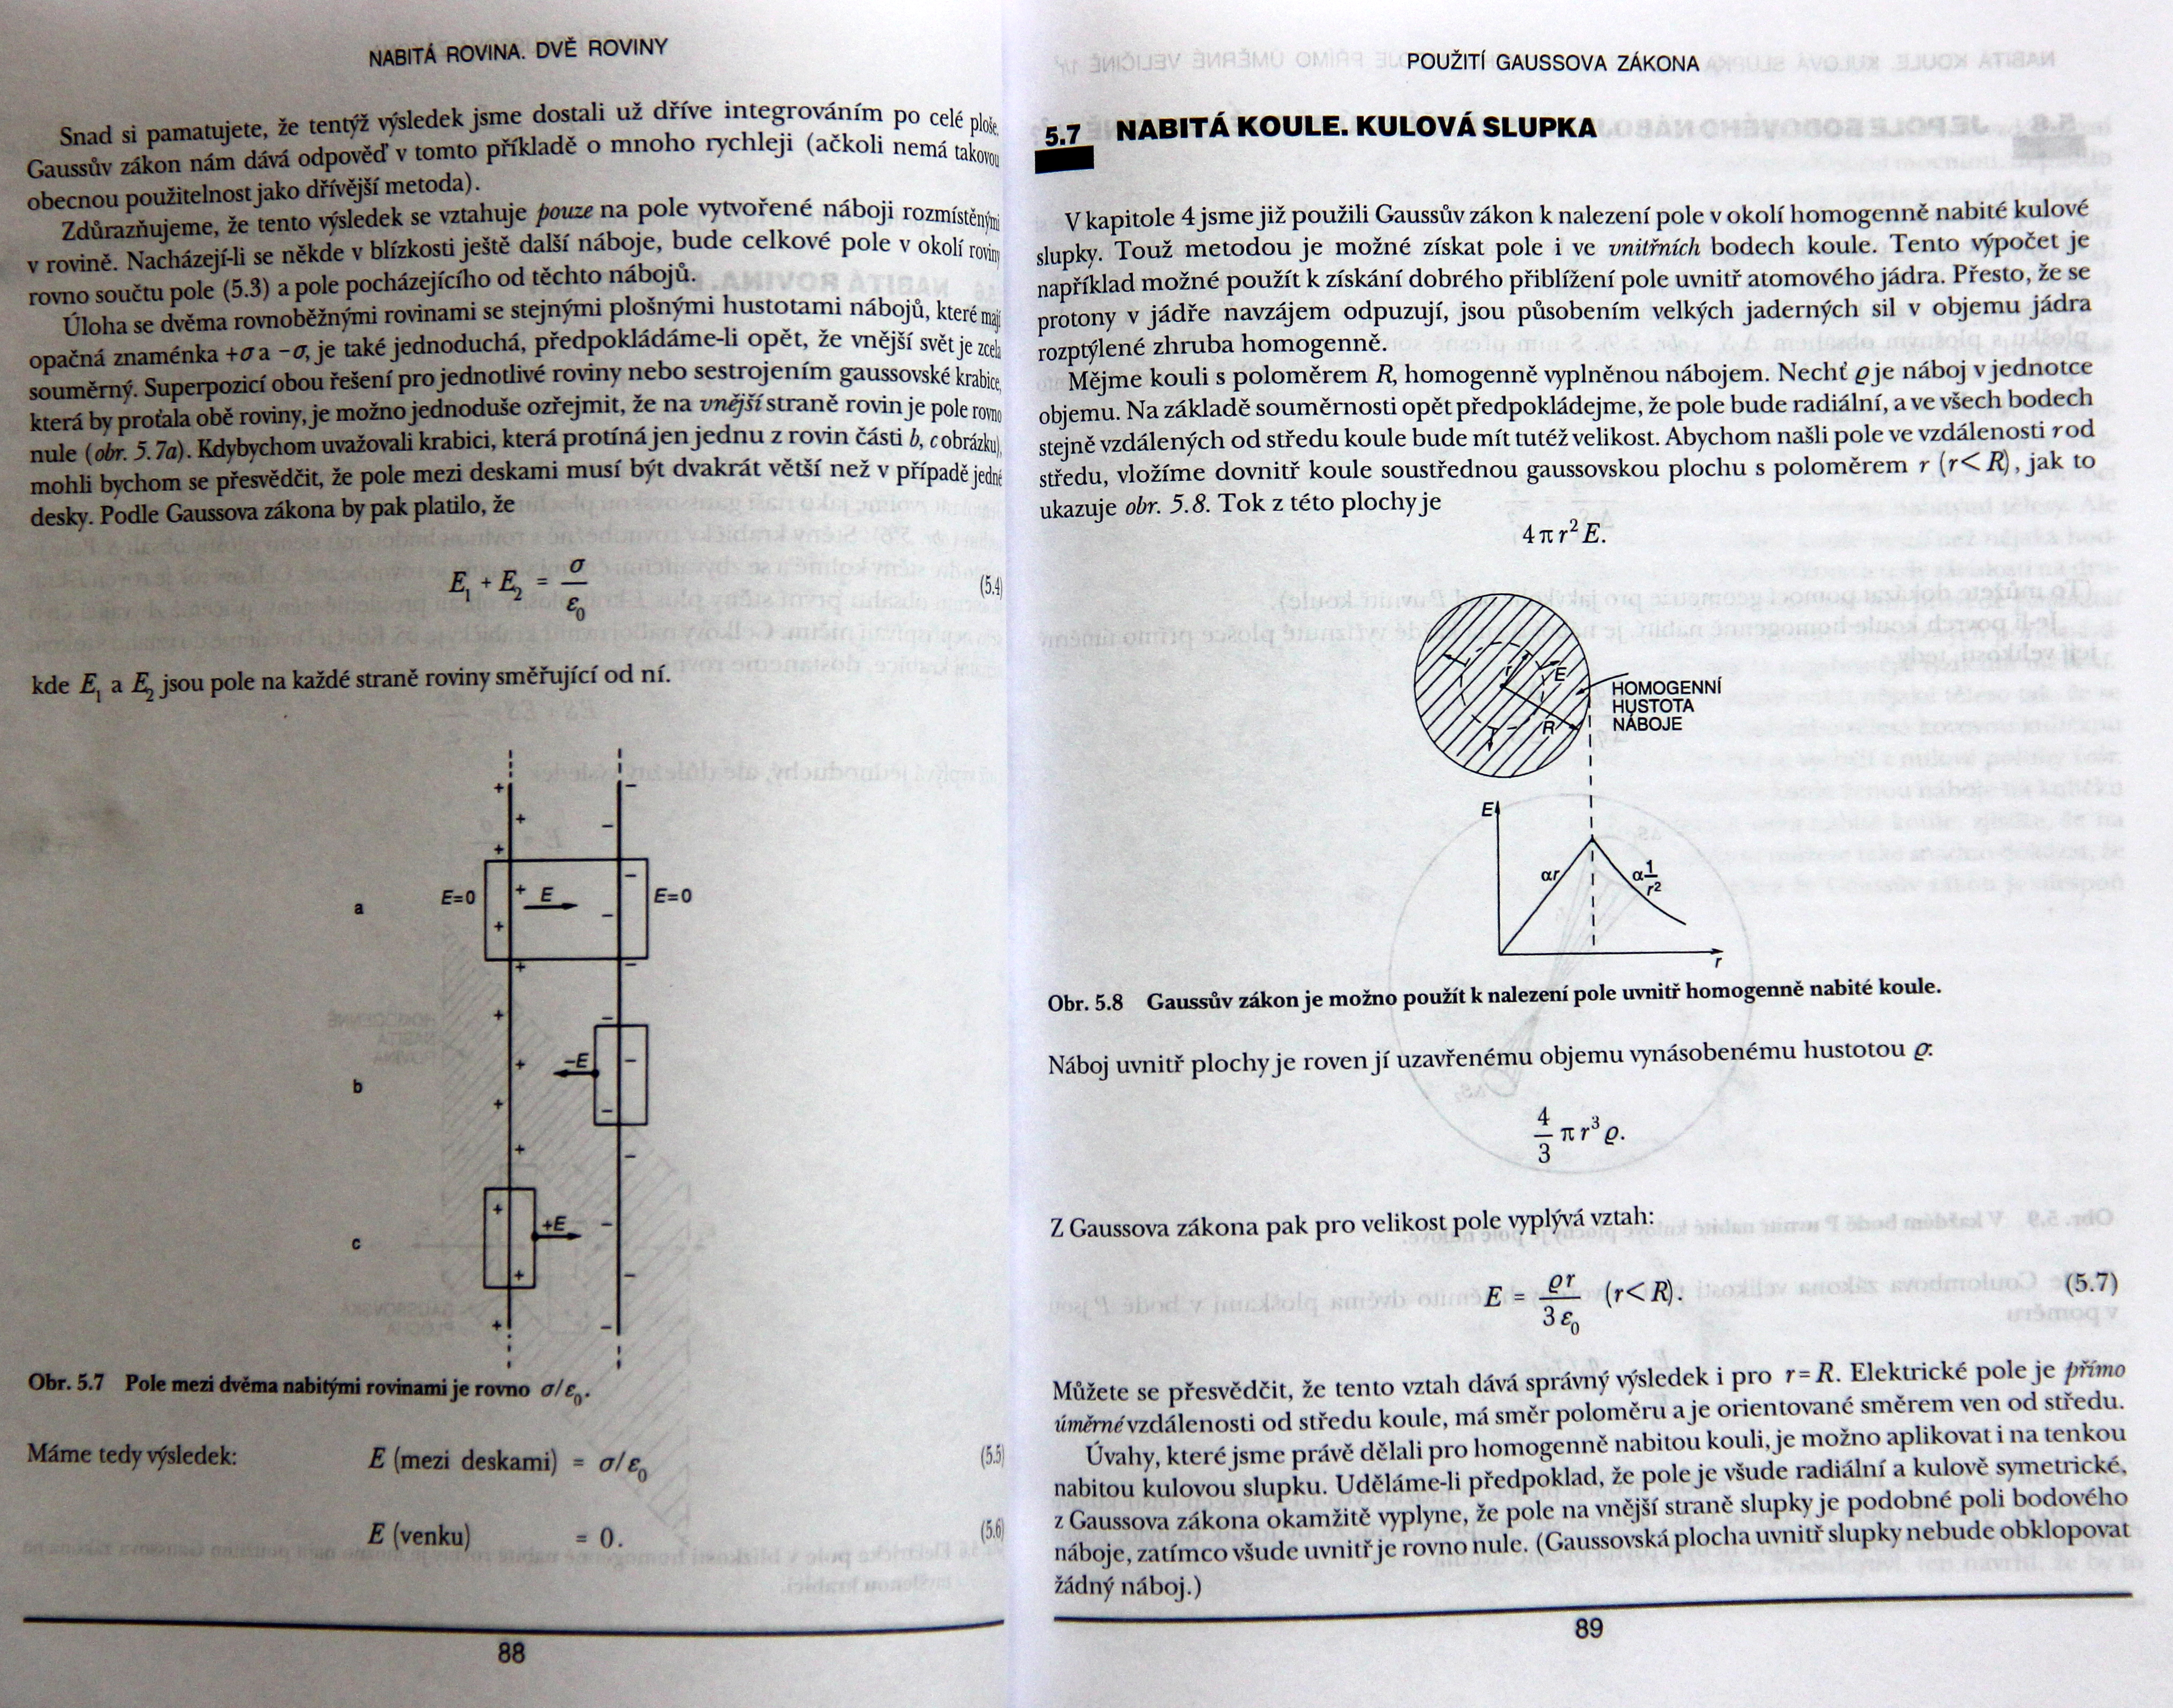
\includegraphics[width=0.6\linewidth]{fey_elstat_gauss08.jpg}
        \caption{Gaussův zákon je možno použít k nalezení pole uvnitř homogenně nabité koule.}
        \label{fyz:fig_fey_elstat_gauss08}
      \end{figure}
      Náboj uvnitř plochy je roven jí uzavřenému objemu vynásobenému hustotou \(\varrho\):
      \begin{align}
        Q_{\text{uvnitř}} 
                = \limitint_{\mathclap{\substack{\text{objem}\\
                                                 \text{uvnitř }S}}} \varrho\dd{V} 
          &= \frac{4}{3}\pi r^3\varrho.    \label{fyz:eq_fey_elstat_gauss05}    \\
       \shortintertext{Z Gaussova zákona pak pro velikost pole vyplývá vztah:}
       \limitint_S E_n\dd{S}
          &= \frac{Q_{\text{uvnitř}}}{\varepsilon_0} 
                \qquad\Rightarrow\qquad 4\pi r^2E 
                = \frac{4\pi r^3\varrho}{3\,\varepsilon_0}  \label{fyz:eq_fey_elstat_gauss06} \\ 
       \shortintertext{tedy:}
       E  &= \frac{\varrho r}{3\,\varepsilon_0} \qquad (r<R).
      \end{align}
      
      Můžete se přesvědčit, že tento vztah dává správný výsledek i pro \(r=R\). Elektrické pole je přímo 
      úměrné vzdálenosti od středu koule, má směr poloměru a je orientované směrem ven od středu.
      Úvahy, které jsme právě dělali pro homogenně nabitou kouli, je možno aplikovat i na tenkou nabitou 
      kulovou slupku. Uděláme-li předpoklad, že pole je všude radiální a kulově symetrické, z Gaussova zákona 
      okamžitě vyplyne, Že pole na vnější straně slupky je podobné poli bodového náboje, zatímco všude 
      uvnitř je rovno nule. (Gaussovská plocha uvnitř slupky nebude obklopovat žádný náboj.)
      
    \subsection{Je pole bodového náboje přesně přímo úměrné veličině 
                 \texorpdfstring{\(\frac{1}{r^2}\)}{1/r^2}?} 
      Podíváme-li se trochu podrobněji, jak se pole uvnitř kulové slupky stává nulovým, lépe si ozřejmíme, 
      proč platnost Gaussova zákona vyplývá právě jen z přesné závislosti Coulombovy síly na druhé mocnině 
      vzdálenosti. Uvažujme nějaký bod \(P\) uvnitř homogenně nabité kulové plochy. Představme si úzký kužel, 
      který má vrchol v \(P\) a sahá po kulovou plochu, na které vytíná malou plošku s plošným obsahem 
      \(\Delta S_1\) (obr. \ref{fyz:fig_fey_elstat_gauss09}). S ním přesně souměrný kužel vycházející z \(P\) 
      na opačnou stranu by na kulové ploše vyřízl plošku s obsahem \(\Delta S_2\). Jsou-li vzdálenosti od 
      \(P\) k těmto dvěma ploškám \(r_1\) a \(r_2\), jsou jejich plošné obsahy v poměru \[\frac{\Delta 
      S_2}{\Delta S_1} = \frac{r_2^2}{r_1^2}\]
      (To můžete dokázat pomocí geometrie pro jakýkoliv bod \(P\) uvnitř koule).
      
      Je-li povrch koule homogenně nabitý, je náboj \(\Delta q\) na každé vyříznuté plošce přímo úměrný její 
      velikosti, tedy \[\frac{\Delta q_2}{\Delta q_1} = \frac{\Delta S_2}{\Delta S_1}.\]
      
      
      \begin{figure}[ht!] % \ref{fyz:fig_fey_elstat_gauss09}
        \centering
        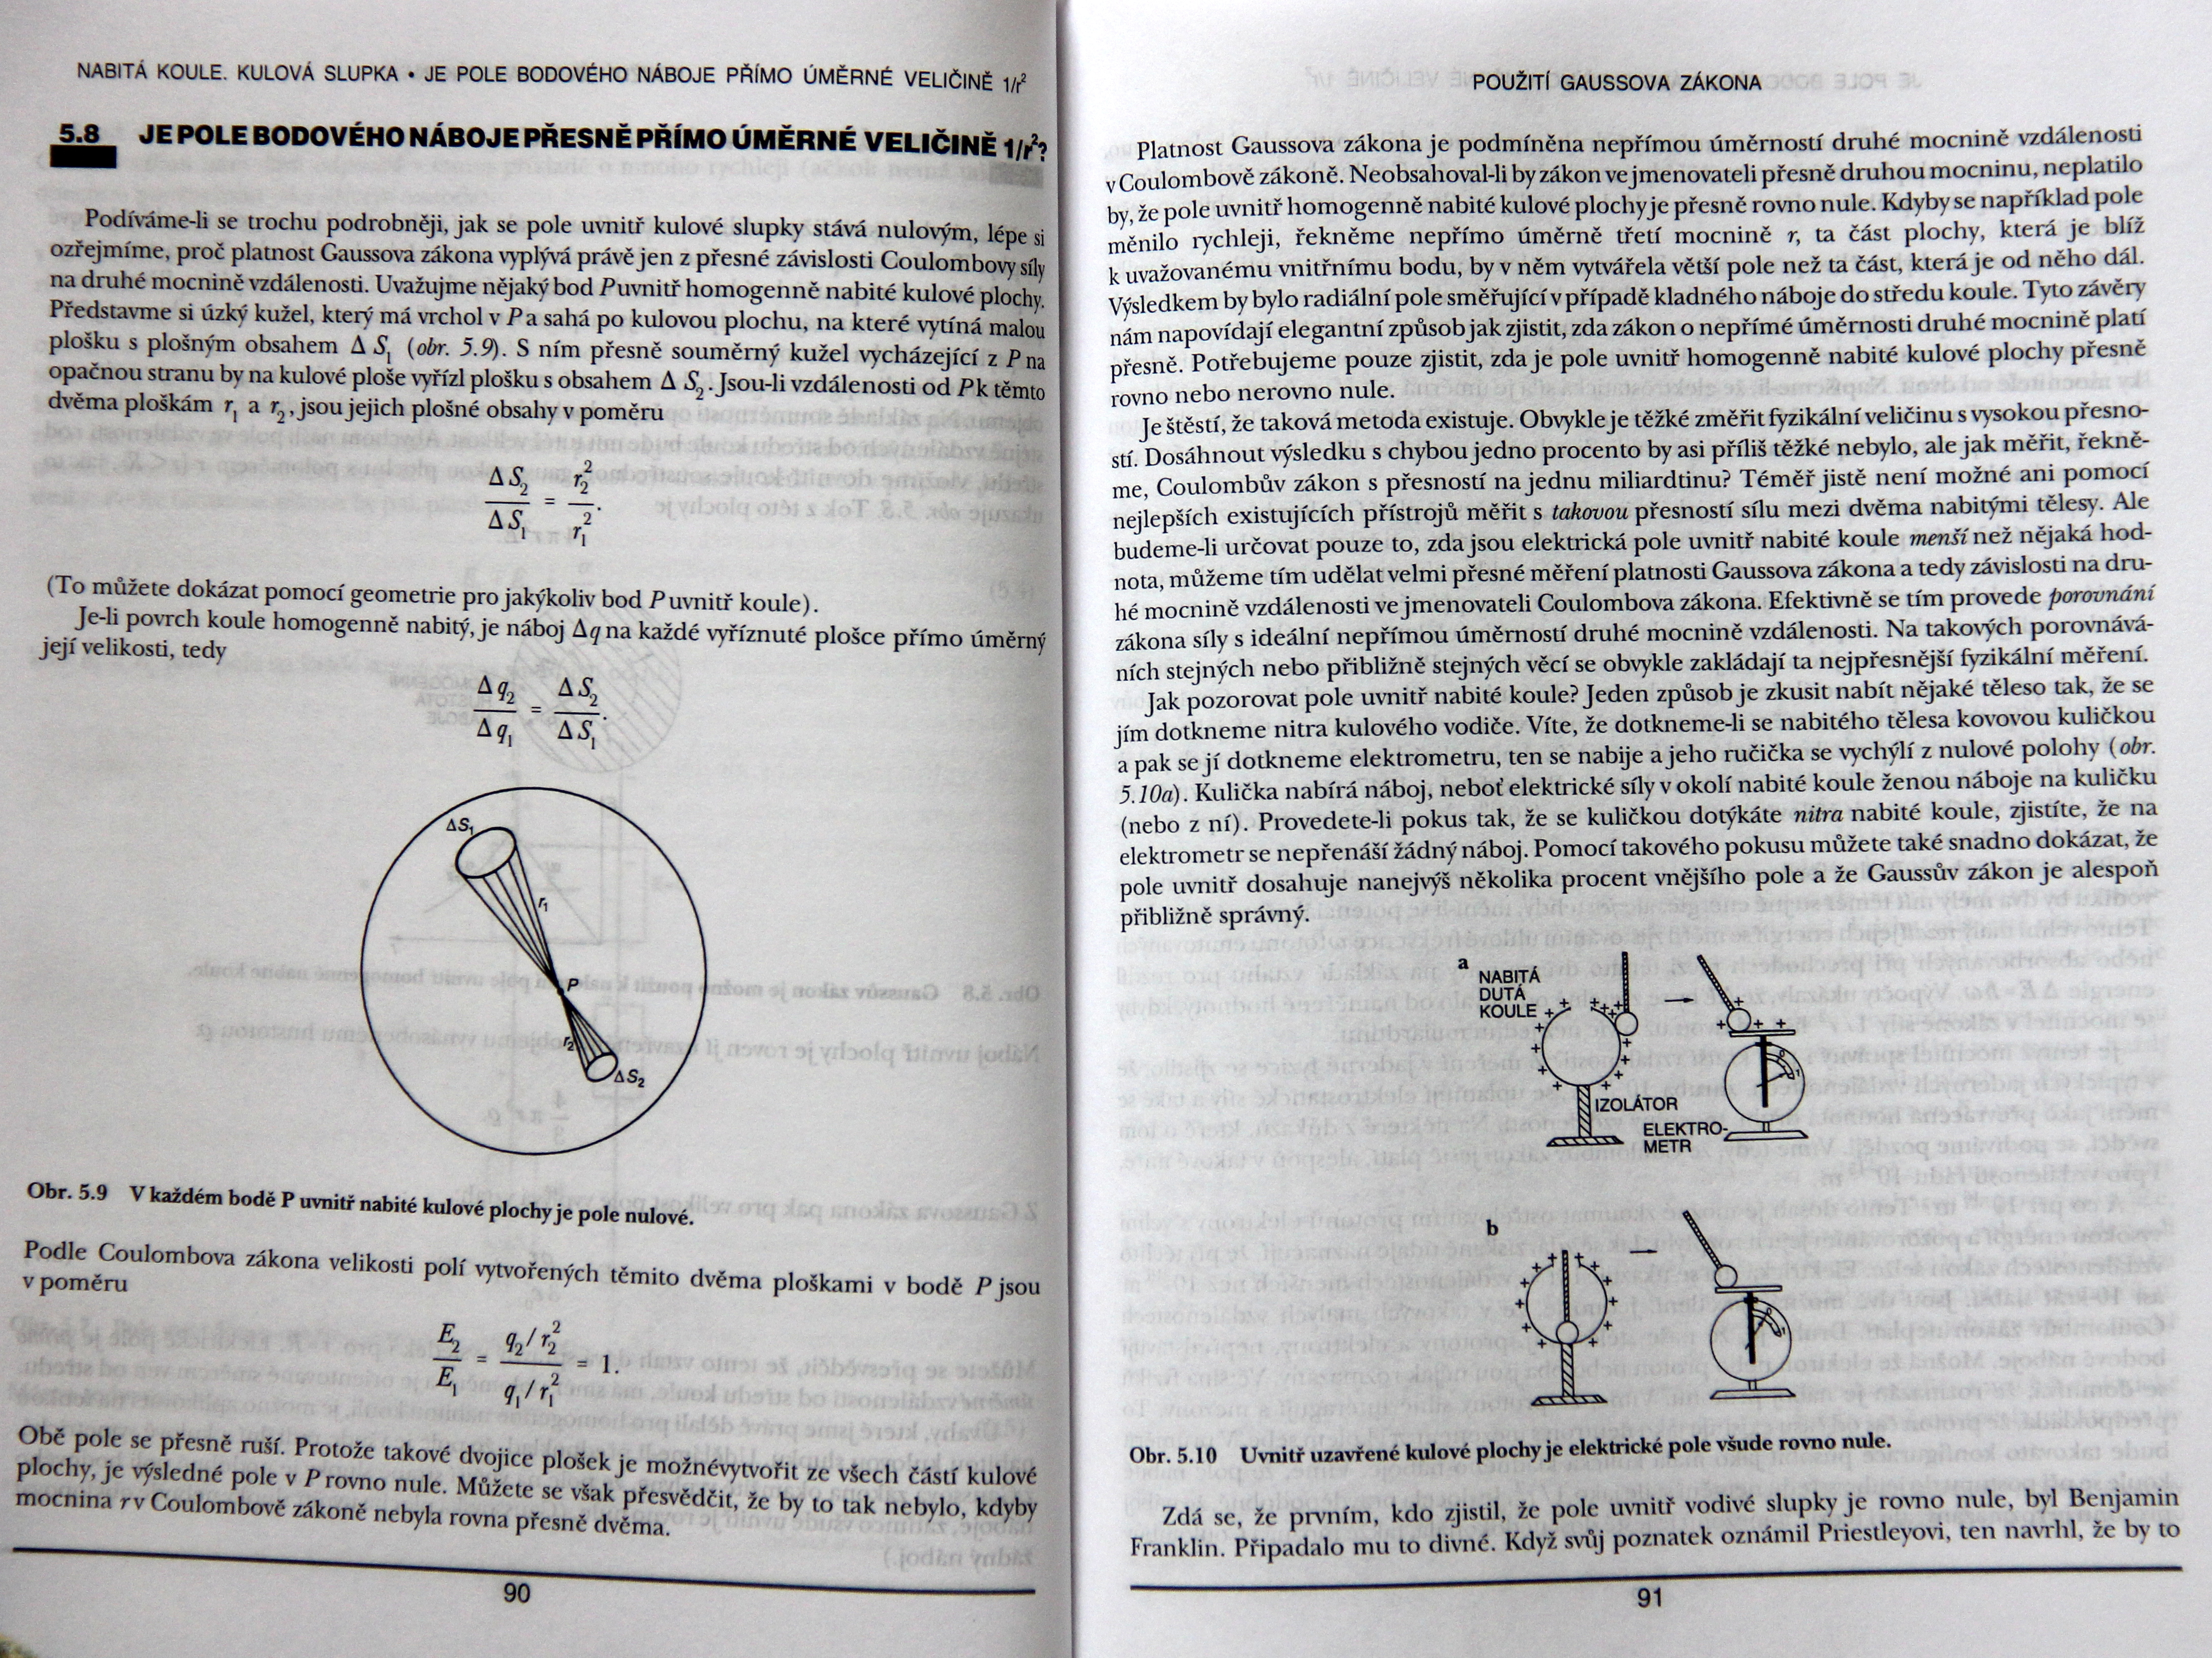
\includegraphics[width=0.6\linewidth]{fey_elstat_gauss09.jpg}
        \caption{V každém bodě \(P\) uvnitř nabité kulové plochy je pole nulové.}
        \label{fyz:fig_fey_elstat_gauss09}
      \end{figure}
      
      Podle Coulombova zákona velikosti polí vytvořených těmito dvěma ploškami v bodě \(P\) jsou v poměru
      \[\frac{E_2}{E_1} = \frac{q_2/r_2^2}{q_1/r_1^2} = 1.\]
      
      Obě pole se přesně ruší. Protože takové dvojice plošek je možné vytvořit že všech Částí kulové plochy, 
      je výsledné pole v \(P\) rovno nule. Můžeme se však přesvědčit, že by to tak nebylo, kdyby mocnina 
      \(r\) v Coulombově zákoně nebyla rovna přesně dvěma.
      
      Platnost Gaussova zákona je podmíněna nepřímou úměrností druhé mocnině vzdálenosti v Coulombově zákoně. 
      Neobsahoval-li by zákon ve jmenovateli přesně druhou mocninu, neplatilo by, že pole uvnitř homogenně 
      nabité kulové plochy je přesně rovno nule. Kdyby se například pole měnilo rychleji, řekněme nepřímo 
      úměrně třetí mocnině \(r\), ta část plochy, která je blíž k uvažovanému vnitřnímu bodu, by v něm 
      vytvářela větší pole než ta část, která je od něho dál. Výsledkem by bylo radiální pole směřující v 
      případě kladného náboje do středu koule. Tyto závěry nám napovídají elegantní způsob jak zjistit, zda 
      zákon o nepřímé úměrnosti druhé mocnině platí přesně. Potřebujeme pouze zjistit, zda je pole uvnitř 
      homogenně nabité kulové plochy přesně rovno nebo nerovno nule.
      
      Je štěstí, že taková metoda existuje. Obvykle je těžké změřit fyzikální veličinu s vysokou přesností. 
      Dosáhnout výsledku s chybou jedno procento by asi příliš těžké nebylo, ale jak měřit, řekněme, 
      Coulombův zákon s přesností na jednu miliardtinu? Téměř jistě není možné ani pomocí nejlepších 
      existujících přístrojů měřit s takovou přesností sílu mezi dvěma nabitými tělesy. Ale budeme-li určovat 
      pouze to, zda jsou elektrická pole uvnitř nabité koule menší než nějaká hodnota, můžeme tím udělat 
      velmi přesné měření platnosti Gaussova zákona a tedy závislosti na druhé mocnině vzdálenosti ve 
      jmenovateli Coulombova zákona. Efektivně se tím provede porovnání zákona síly s ideální nepřímou 
      úměrností druhé mocnině vzdálenosti. Na takových porovnáváních stejných nebo přibližně stejných věcí 
      se obvykle zakládají ta nejpřesnější fyzikální měření.
      
      Jak pozorovat pole uvnitř nabité koule? Jeden způsob je zkusit nabít nějaké těleso tak, že se jím 
      dotkneme nitra kulového vodiče. Víte, že dotkneme-li se nabitého tělesa kovovou kuličkou a pak sejí 
      dotkneme elektrometru, ten se nabije a jeho ručička se vychýlí z nulové polohy (obr 
      \ref{fyz:fig_fey_elstat_gauss10}). Kulička nabírá náboj, neboť elektrické síly v okolí nabité koule 
      ženou náboje na kuličku (nebo z ní). Provedeme-li pokus tak, že se kuličkou dotýkáte nitra nabité 
      koule, zjistíme, že na elektrometr se nepřenáší žádný náboj. Pomocí takového pokusu můžete také snadno 
      dokázat, že pole uvnitř dosahuje nanejvýš několika procent vnějšího pole a že Gaussův zákon je alespoň 
      přibližné správný \cite[s.~91]{Feynman02}.
      \begin{figure}[hb!]
        \centering
        \begin{tabular}{cc}
         \subfloat[ ]{\label{fyz:fig_fey_elstat_gauss10}
           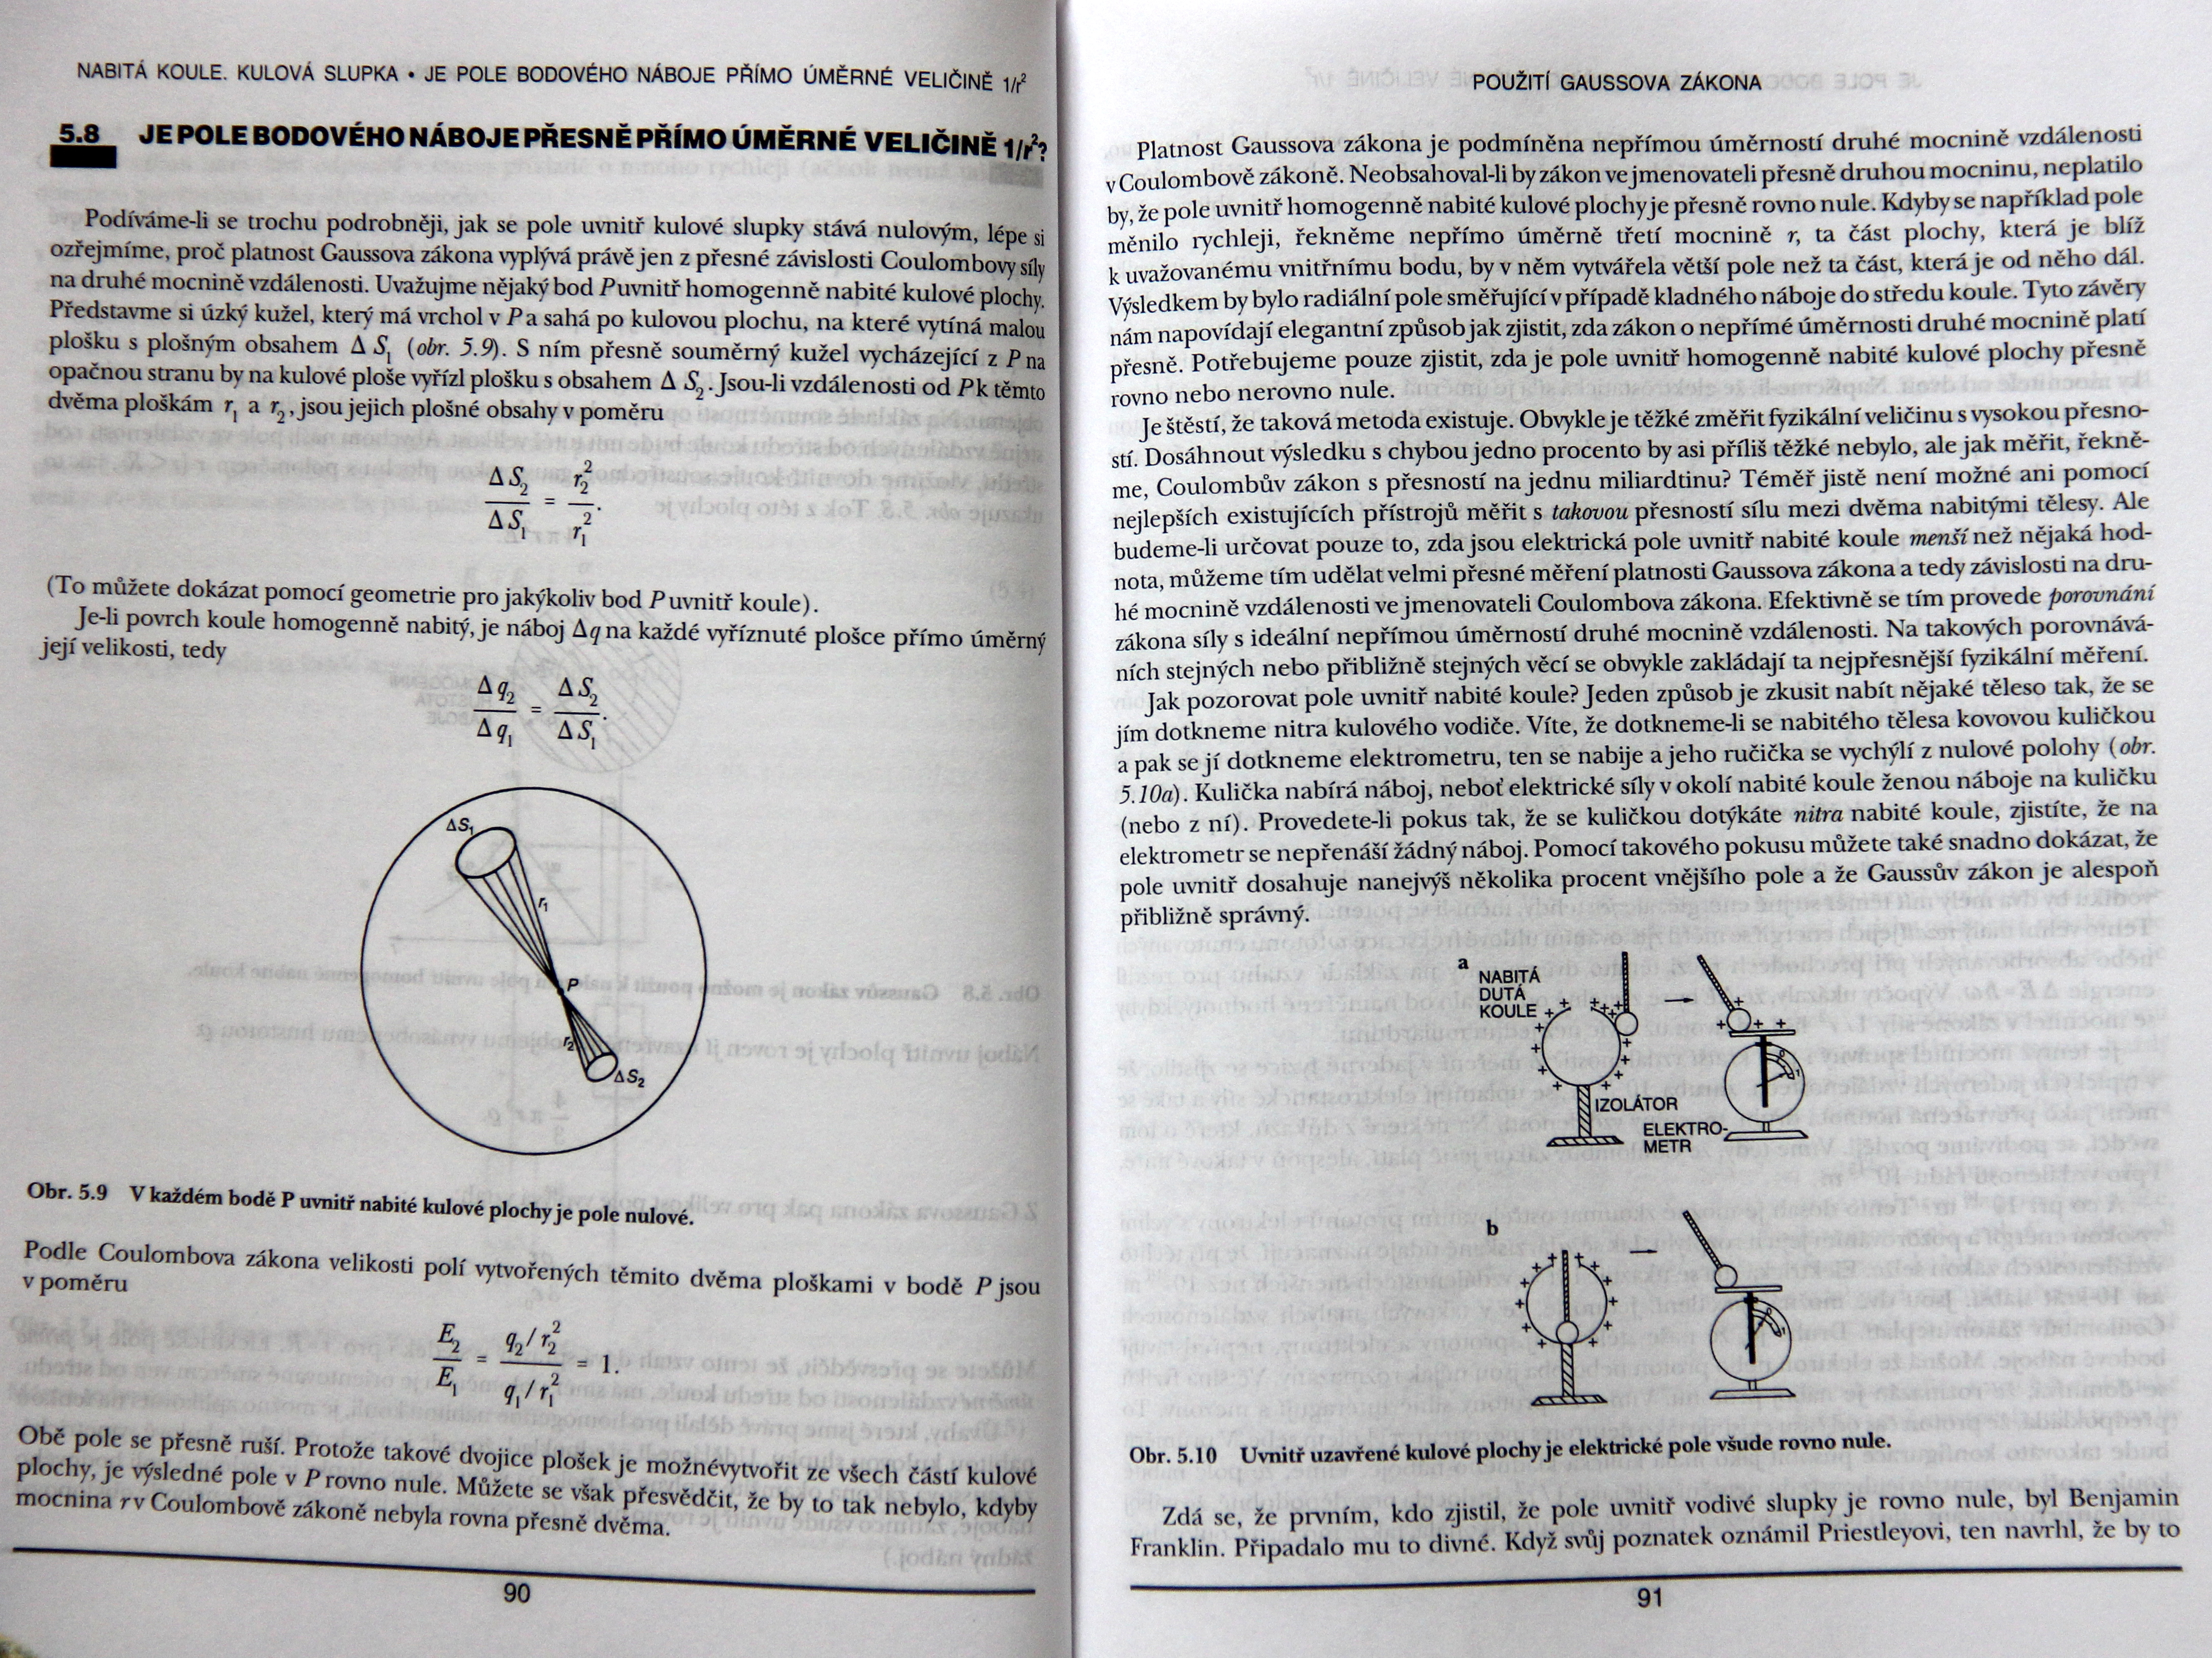
\includegraphics[width=0.2\textwidth]{fey_elstat_gauss10.jpg}}              &
         \subfloat[ ]{\label{fyz:fig_fey_elstat_gauss11}
           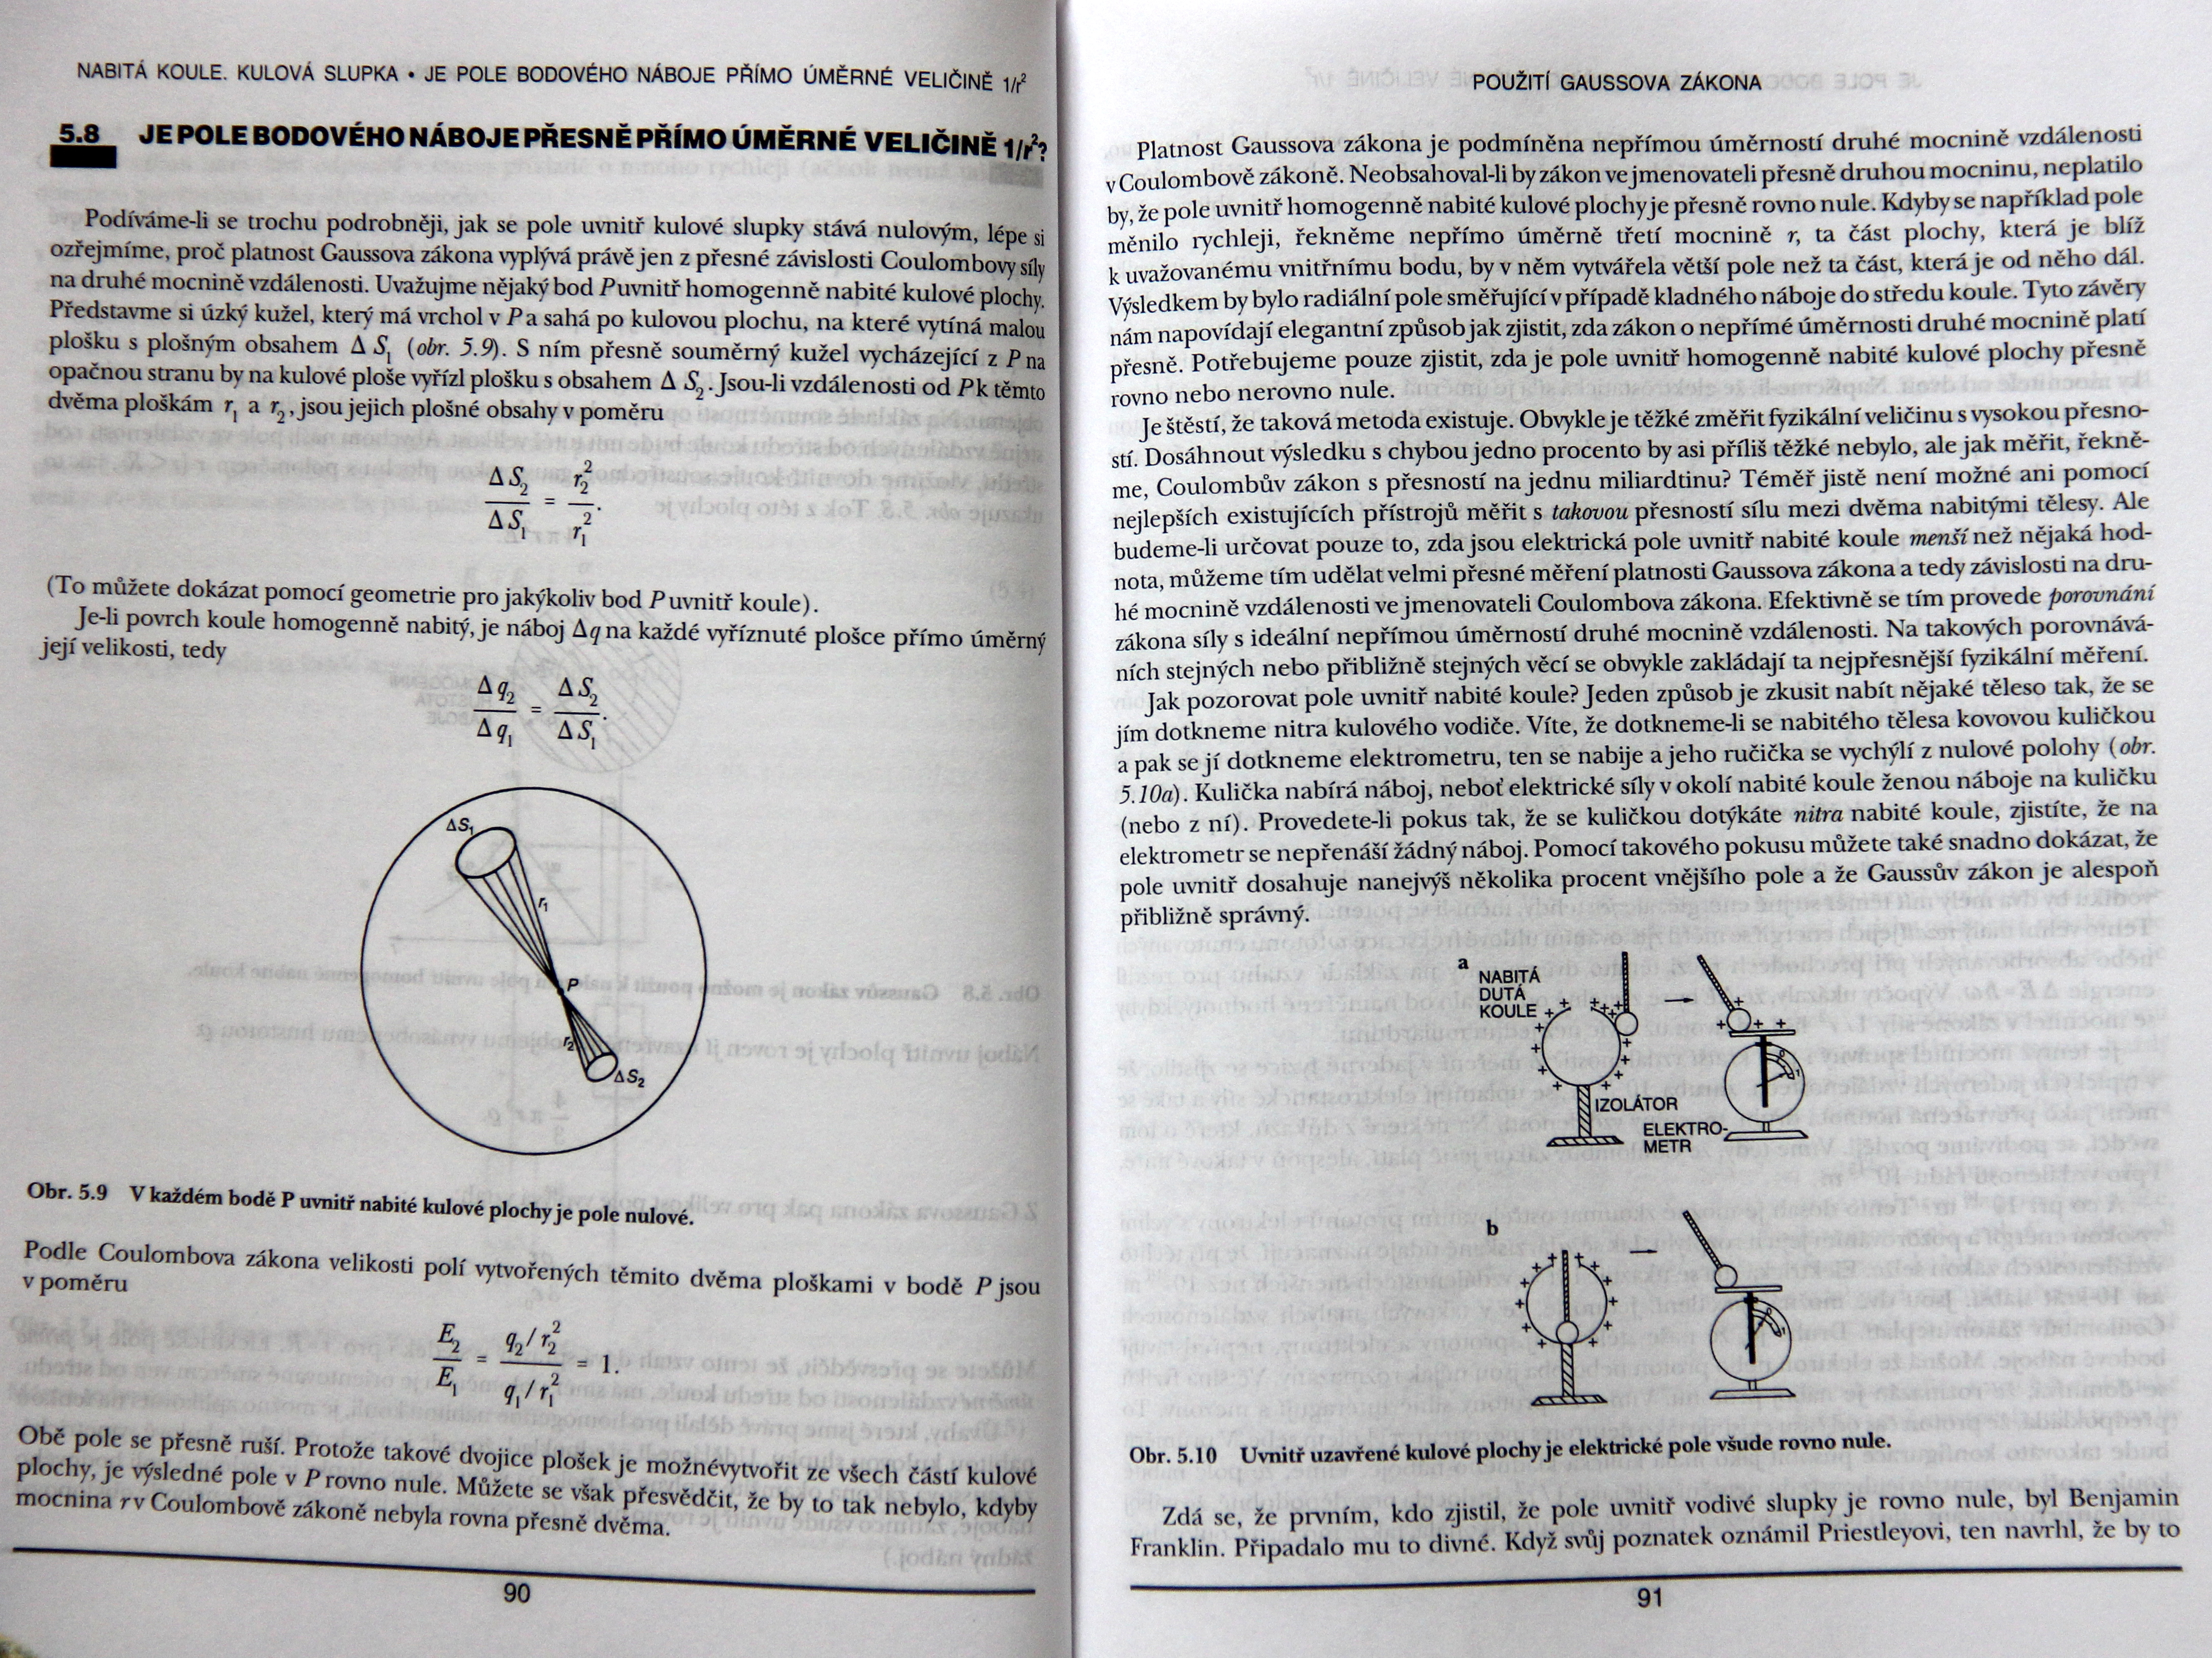
\includegraphics[width=0.2\textwidth]{fey_elstat_gauss11.jpg}}                        \\
        \end{tabular}                          
        \caption{Uvnitř uzavřené kulové plochy je elektrické pole všude rovno nule.}
        \label{fyz:fig_fey_elstat_gauss_koule}
      \end{figure}       
        
      Zdá se, že prvním, kdo zjistil, že pole uvnitř vodivé slupky je rovno nule, byl Benjamin Franklin. 
      Připadalo mu to divné. Když svůj poznatek oznámil Priestleyovi, ten navrhl, že mohlo souviset se 
      zákonem nepřímé úměrnosti druhé mocnině vzdálenosti, neboť bylo známo, že kulová hmotná slupka uvnitř 
      nevytváří žádné gravitační pole. Ale Coulomb naměřil nepřímou úměrnost druhé mocnině vzdálenosti až o 
      18 let později a Gaussův zákon byl objeven ještě později.
      
      Gaussův zákon byl pečlivě prověřován. Za tímto účelem se elektrometr umístil uvnitř velké koule a 
      sledovalo se, zda se neobjeví nějaké výchylky, když se koule nabije na vysoké napětí. Vždy bylo 
      dosaženo záporného výsledku. Z geometrie aparatury a citlivosti elektrometru je možné vypočítat, jaké 
      nejmenší pole by se projevilo. Z této hodnoty lze stanovit horní ohraničení odchylky mocnitele od dvou. 
      Napíšeme-li, že elektrostatická síla je úměrná \(r^{2+\varepsilon}\), můžeme určit horní hranici pro 
      \(\varepsilon\). Touto metodou Maxwell určil, že \(\varepsilon\) je méně než \(\num{1/10 000}\). V roce 
      1936 Plimpton a Laughton experiment zopakovali a zdokonalili. Zjistili, že mocnitel se liší od dvou o 
      méně než jednu miliardtinu.
      
      To nás přivádí k zajímavé otázce: Do jaké míry víme, jak přesně platí Coulombův zákon v různých 
      situacích? Právě popsané pokusy měří závislost pole na vzdálenosti řekněme několika desítek centimetrů. 
      Ale co třeba vzdálenosti uvnitř atomu, např. vodíkového atomu, v němž, jak předpokládáme, je elektron 
      přitahován k jádru podle téhož zákona nepřímé úměrnosti druhé mocnině vzdálenosti? Je pravda, že k 
      popisu mechanické stránky chování elektronu musí být použita kvantová mechanika, ale přitom jde o 
      obyčejnou elektrostatickou sílu. Při formulování úlohy o atomu vodíku je potřeba znát potenciální 
      energii elektronu jako funkci vzdálenosti od jádra. Coulombův zákon dává potenciál, který se mění 
      nepřímo úměrně první mocnině vzdálenosti. S jakou přesností je znám mocnitel pro takové malé 
      vzdálenosti? Z velmi pečlivých měření relativních poloh energetických hladin vodíku, které provedli 
      Lamb a Retherford r. 1947, víme, že v rozměrech atomu, tj. ve vzdálenostech řádově desetin nanometru 
      (\SI{10e-10}{\meter}), Souhlasí mocnitel opět s přesností jedné miliardtiny.
      
      Přesnost Lambova-Retherfordova měření znovu umožnila fyzikální „náhoda“. Ze stavů atomu vodíku by dva 
      měly mít téměř stejné energie, ale jen tehdy, mění-li se potenciál přesně jako \(1/r\). Tento velmi 
      malý rozdíl jejich energií se měřil zjišťováním úhlové frekvence \(\omega\) fotonů emitovaných nebo 
      absorbovaných při přechodech mezi těmito dvěma stavy na základě vztahu pro rozdíl energie \(\Delta E 
      = \si{\planckbar}\omega\)). Výpočty ukázaly, že \(\delta E\) by se zřetelně odlišovalo od naměřené 
      hodnoty, kdyby se mocnitel v zákoně síly \(1/r^2\) lišil od dvou už o víc než jednu miliardtinu.
      
      Je tentýž mocnitel správný i pro kratší vzdálenosti? Z měření v jaderné fyzice se zjistilo, že v 
      typických jaderných vzdálenostech, zhruba \SI{10e-15}{\meter}, se uplatňují elektrostatické síly a také 
      se mění jako převrácená hodnota druhé mocniny vzdálenosti. Na některé z důkazů, které o tom svědčí, se 
      podíváme později. Víme tedy, že Coulombův zákon ještě platí, alespoň v takové míře, i pro vzdálenosti 
      řádu \SI{10e-10}{\meter}.
      
      A co při \SI{10e-16}{\meter}? Tento dosah je možné zkoumat ostřelováním protonů elektrony s velmi 
      vysokou energií a pozorováním jejich rozptylu. Jak se zdá, získané údaje naznačují, že při těchto 
      vzdálenostech zákon selže. Elektrická síla se ukazuje být ve vzdálenostech menších než 
      \SI{10e-16}{\meter} asi 10-krát slabší. Jsou dvě možná vysvětlení. Jedno je, že v takových malých 
      vzdálenostech Coulombův zákon neplatí. Druhé je, že naše „tělesa“, tj. protony a elektrony, 
      nepředstavují bodové náboje. Možná že elektron nebo proton nebo oba jsou nějak rozmazány. Většina 
      fyziků se domnívá, že rozmazán je náboj protonu. Víme, že protony silně interagují s mezony. To 
      předpokládá, že proton čas od času existuje jako neutron s mezonem \(\pi^+\) kolem sebe. V průměru bude 
      takováto konfigurace působit jako malá kulička kladného náboje. Víme, že pole nabité koule se při 
      postupu do jejího středu nemění stále jako \(1/r^2\). Je docela pravděpodobné, že náboj protonu je 
      rozmazaný, ale i teorie \(\pi\text{-mezonů}\) je ještě dost nedokonalá, takže možná i Coulombův zákon 
      selže na velmi malých vzdálenostech\footnote{Experimenty, které Feynman popisuje, postupně vedly k 
      dnešní představě, podle níž protony, neutrony i mezony skutečně nejsou bodové částice, ale mají vnitřní 
      strukturu tvořenou kvarky. Kvarky přitom nemohou existovat samostatně.}.
      
      Ještě jedna věc: zákon nepřímé úměrnosti druhé mocnině vzdáleností platí pro vzdálenosti řádu 
      \SI{1}{\meter}, ale i pro \SI{10e-10}{\meter}; zůstává však činitel \(\dfrac{1}{4\pi\varepsilon_0}\) 
      stále stejným? Odpověď je ano, alespoň s relativní přesností 15 milióntin.
      
      Nyní se vraťme k důležitému problému, který jsme přešli mlčením, když jsme hovořili o experimentálním 
      potvrzení Gaussova zákona. Možná, že jste se podivili, jak mohl být výsledek experimentu Maxwella nebo 
      Plimptona a Lauglitona tak přesný, když přitom kulový vodič, který použili, nebyl dokonalou koulí. 
      Vždyť dosáhnout přesnosti na jednu miliardtinu je už opravdu něco a právem byste se mohli ptát, zda 
      dokázali udělat tak přesnou kouli. Každá reálná koule má určitě malé nepravidelností. Existují-li 
      nepravidelnosti, nebudou uvnitř vytvářet pole? Nyní chceme ukázat, že není třeba mít dokonalou kouli. 
      Opravdu lze dokázat, že uvnitř uzavřené vodivé plochy jakéhokoliv tvaru není žádné pole. Jinými slovy, 
      výsledek zmíněných experimentů závisel na \(1/r^2\), ale vůbec ne na tom, zda je plocha kulová (až na 
      to, že pro kouli je snazší vypočítat, jaká by byla pole, kdyby Coulombův zákon neplatil), a tak se nyní 
      vracíme znovu k našemu problému. Abychom to ukázali, je nevyhnutelné poznat některé vlastností 
      elektrických vodičů.
      
    \subsection{Pole vodiče}
      Elektrickým vodičem je pevné těleso, které obsahuje mnoho „volných“ elektronů. Elektrony se mohou v 
      tělese volně pohybovat, ale nemohou projít jeho povrchem. V kovu je tolik volných elektronů, že 
      jakékoliv elektrické pole jich uvede do pohybu velké množství. Takto vzniklý proud elektronů se pak 
      musí buď udržovat vnějšími zdroji energie, nebo se pohyb elektronů zastaví, jakmile elektrony vybijí 
      zdroje, které vytvořily původní pole. V elektrostatice nepracujeme se stálými zdroji proudu (jimi se 
      budeme zabývat později, až budeme hovořit o magnetostatice), takže elektrony se pohybují jen dokud se 
      neuspořádají tak, aby všude uvnitř vodiče vytvořily nulové elektrické pole. (Obvykle se to stane v 
      malém zlomku sekundy). Kdyby totiž ještě nějaké pole zůstalo, uvedlo by do pohybu další elektrony; 
      jediným možným řešením v elektrostatice je, že je pole uvnitř vodiče je všude nulové.
      
      Nyní si všimněme vnitřku nabitého vodivého tělesa. („Vnitřkem“ rozumíme prostor v objemu kovu.) Protože 
      kov je vodič, vnitřní pole, a tedy gradient potenciálu \(\varphi\) musí být roven nule. Každý vodič tak 
      představuje ekvipotenciální oblast a jeho povrch je ekvipotenciální plochou. Protože všude ve vodivé 
      látce je elektrické pole rovno nule, je nule rovna i divergence \(\vec{E}\) a podle Gaussova zákona 
      musí být rovna nule i hustota náboje uvnitř vodiče.
      
      Nemohou-li být ve vodiči žádné náboje, jak je možné jej nabít? Co máme na mysli, když říkáme, že je 
      vodič „nabit“? Kde tedy náboje jsou? Odpověď je, že se nacházejí na povrchu vodiče, kde působí velké 
      síly, které jim zabraňují uniknout, tedy náboje nejsou zcela „volné“. Budeme-li studovat fyziku pevných 
      látek, dozvíme se, že přebytečný náboj se v každém vodiči nachází v jedné - dvou atomových vrstvách 
      povrchu. Pro naše současné účely je dostačující přesnost říkat, že převede-li se nějaký náboj na vodič 
      nebo do něj, celý se shromáždí na jeho povrchu; uvnitř vodiče žádné náboje nejsou.
      
      Kromě toho si všimněte, že na vnější straně v těsné blízkosti povrchu vodiče musí být elektrické pole 
      kolmé na povrch. Nemůže existovat žádná tečná složka. Kdyby totiž existovala, elektrony by se 
      pohybovaly podél povrchu; neexistují žádné síly, které by jim v tom zabraňovaly. Jinými slovy víme, že 
      elektrické siločáry musí vždy svírat s ekvipotenciální plochou pravý úhel.
      
      Na základě Gaussova zákona můžeme také uvést do vztahu intenzitu pole blízko povrchu vodiče s lokální 
      hustotou náboje na jeho povrchu. Jako gaussovskou plochu vezmeme malou válcovou krabičku jednou 
      polovičkou pod a druhou polovičkou nad povrchem (obr. \ref{fyz:fig_fey_elstat_gauss12}). K celkovému 
      toku \(\vec{E}\) přispívá pouze ta strana krabičky, která je mimo vodič. Pole těsně při povrchu vodiče 
      z jeho vnější strany je potom
      \begin{figure}[ht!] % \ref{fyz:fig_fey_elstat_gauss12}
        \centering
        \includegraphics[width=0.4\linewidth]{fey_elstat_gauss12.png}
        \caption{Elektrické pole těsně při povrchu vodiče je přímo úměrné lokální plošné hustotě náboje na 
                 povrchu.}
        \label{fyz:fig_fey_elstat_gauss12}
      \end{figure} 
      Vně vodiče
      \begin{equation}\label{fyz:eq_fey_elstat_gauss07}
        E = \frac{\sigma}{\varepsilon_0}  \qquad\text{\(\sigma\ldots\) lokální plošná hustota náboje}.
      \end{equation}
      
      Proč nabitá vrstva na povrchu náboje vytváří jiné pole než samotná nabitá rovina? Jinými slovy, proč je 
      (\ref{fyz:eq_fey_elstat_gauss07}) dvakrát větší než (\ref{fyz:eq_fey_elstat_gauss03})? Důvod spočívá, 
      samozřejmě, v tom, že v případě vodiče jsme netvrdili, že se v okolí nenacházejí žádné „jiné“ náboje. 
      Opravdu nějaké ještě musí být, aby ve vodiči bylo \(\vec{E} = 0\). Náboje, nacházející se v 
      bezprostředním sousedství bodu \(P\) na povrchu vodiče, ve skutečnosti vytvářejí pole 
      \(E_{lok}=\frac{\sigma_{lok}}{2\varepsilon_0}\) jak z vnitřní tak i z vnější strany povrchu. Ale všechny
      ostatní náboje na vodiči se „spikly“, aby vytvořily v bodě \(P\) dodatkové pole s velikostí 
      \(E_{lok}\). Výsledné vnitřní pole je pak nulové a vnější je rovno \(2E_{lok} = 
      \frac{\sigma_{lok}}{\varepsilon_0}\) \cite[s.~93]{Feynman02}.
      
    \subsection{Pole vodiče}
      Nyní se vrátíme k problému duté schránky - vodiči s dutinou. Uvnitř kovu není žádné pole, ale jak tomu 
      bude v dutině? Ukážeme, že je-li dutina prázdná, pak v ní pole nejsou bez ohledu na to, jaký tvar má 
      vodič nebo dutina. Ukážeme to například pro tvar na obr. \ref{fyz:fig_fey_elstat_gauss13}. Uvažujme 
      gaussovskou plochu takového tvaru, jaký má plocha \(S\) vyznačená na obr. 
      \ref{fyz:fig_fey_elstat_gauss13}, která obklopuje dutinu, ale všude zůstává ve vodivé látce. Všude na 
      \(S\) je pole rovno nule, takže není žádný tok z \(S\) a celkový náboj uvnitř \(S\) je roven nule. 
      Kdyby šlo o kulovou plochu, by bylo možno ze souměrnosti usoudit, že v jejím nitru by nemohl být žádný 
      náboj. Ale obecně můžeme pouze tvrdit, že na vnitřním povrchu vodiče je stejné množství kladného a 
      záporného náboje. Kladný povrchový náboj by mohl být v jedné jeho části a záporný někde jinde, jako na 
      obr. \ref{fyz:fig_fey_elstat_gauss13}. Gaussovým zákonem není možné něco takového vyloučit.
      \begin{figure}[ht!] % \ref{fyz:fig_fey_elstat_gauss13}
        \centering
        \includegraphics[width=0.4\linewidth]{fey_elstat_gauss13.png}
        \caption{Jaké pole je v prázdné dutině ve vodiči při jakémkoliv tvaru vodiče a dutiny?}
        \label{fyz:fig_fey_elstat_gauss13}
      \end{figure} 
      
      Ve skutečnosti však jakékoliv stejně velké a opačné náboje, nacházející se na vnitřním povrchu, k sobě 
      sklouznou a úplně se vyruší. To, že musí být vyrušeny úplně, můžeme ukázat použitím zákona, že 
      cirkulace pole \(\vec{E}\) je vždy rovna nule (v elektrostatice). Předpokládejme, že by se v některých 
      částech vnitřního povrchu nacházely náboje. Víme, že někde jinde na povrchu by se muselo nacházet 
      stejné množství opačných nábojů. Jakékoliv siločáry pole \(\vec{E}\) by nyní musely vycházet z kladných 
      nábojů a končit v záporných nábojích (neboť uvažujeme pouze o případě, že v dutině nejsou volné 
      náboje). Představme si nyní uzavřenou křivku \(\Gamma\), která prochází napříč dutinou podél některé 
      siločáry od nějakého kladného k některému zápornému náboji a vodičem se vrací zpět do svého výchozího 
      bodu. (jako na obr. \ref{fyz:fig_fey_elstat_gauss13}). Integrál po takové siločáře vedoucí od kladného 
      k zápornému náboji nebude roven nule. Integrál po křivce uvnitř kovu dá však nulu, neboť \(\vec{E}=0\). 
      Dostali jsme tedy že
      \begin{equation}\label{fyz:eq_fey_elstat_gauss08}
        \oint \vec{E}\cdot\dd{\vec{S}} \neq 0  \qquad ???
      \end{equation}
      Křivkový integrál pole \(\vec{E}\) po každé uzavřené křivce je však v elektrostatickém poli roven nule. 
      Z toho vyplývá, že uvnitř prázdné dutiny nemohou existovat žádná pole ani žádné náboje na jejím povrchu.
      
      Měli bychom si pečlivě všimnout důležité výhrady, kterou jsme uvedli. Vždy jsme říkali „uvnitř prázdné“ 
      dutiny. Umístí-li se totiž nějaké náboje do některých pevných poloh v dutině, ať už v izolantu, nebo na 
      malém vodiči izolovaném od hlavního vodivého tělesa, pak se v dutině mohou objevit pole. Ale pak už to 
      není „prázdná“ dutina.
      
      Ukázali jsme, že je-li dutina úplně obklopena vodičem, žádné statické rozdělení nábojů mimo ni nikdy 
      nemůže vytvořit pole v jejím nitru. Tím se vysvětluje princip „stínění“ elektrického zařízení, které 
      je uloženo v kovovém obalu. Stejné úvahy můžeme použít i v důkazu, že žádné statické rozdělení nábojů 
      uvnitř uzavřeného vodiče nemůže vytvořit nějaká pole ve vnějším prostoru. Stínění funguje v obou 
      směrech. V elektrostatice - ne však při proměnných polích - pole na obou stranách uzavřené vodivé 
      plochy jsou úplně nezávislá.
      
      \emph{Nyní chápeme, proč bylo možné prověřit Coulombův zákon s tak velkou přesností. Tvar duté schránky 
      je bezvýznamný. Nemusí být kulový, mohla by to být krychle. Je-li Gaussův zákon přesný, je pole uvnitř 
      vždy nulové. Teď také chápeme, proč je bezpečné sedět uvnitř vysokonapěťové elektrody megavoltového van 
      de Graaffova generátoru bez obavy ze zásahu elektřinou. Umožňuje to Gaussův zákon.}

  %--------------------------------- Elektrické pole v různých případech -------------------------------------
  \section{Elektrické pole v různých případech} 
  
\printbibliography[heading=subbibliography]